% Edit only the text between matching begin and end lines.
\documentclass[11pt,a4paper]{article}
% Shared preamble for TMUA worked solutions. Local edits here are overwritten.

% Reproducible PDFs: no timestamps, no trailer id, no build-path details.
\ifdefined\pdfsuppressptexinfo
  \pdfsuppressptexinfo=-1
  \pdfinfoomitdate=1
  \pdftrailerid{}
\fi

\usepackage{graphicx}
\usepackage{mathtools}
\usepackage{amssymb}
\usepackage{amsmath}
\usepackage{amsthm}
\usepackage{enumitem}
\usepackage{microtype}
\usepackage[table]{xcolor}
\usepackage{array}
\usepackage{booktabs}
\usepackage{tabularx}
\usepackage{longtable}
\usepackage{ragged2e}
\usepackage{fancyhdr}
\usepackage{etoolbox}
\usepackage[
  a4paper,
  left=0.8in,
  right=1in,
  top=1in,
  bottom=0.5in,
  headheight=14pt,
  headsep=0.4in
]{geometry}

\usepackage{pgfplots}
\pgfplotsset{compat=1.18}
\usepgfplotslibrary{fillbetween, polar}
\usetikzlibrary{calc, positioning}
\usetikzlibrary{angles, quotes}
\usetikzlibrary{arrows.meta}
\usetikzlibrary{decorations.pathreplacing, decorations.markings}
\usetikzlibrary{patterns}
\usetikzlibrary{intersections}

\usepackage{tocloft}
\usepackage[hidelinks]{hyperref}
\hypersetup{pdfauthor={danieljsmith.org}, pdfcreator={}, pdfsubject={}, pdfkeywords={}}
\urlstyle{same}
\tocloftpagestyle{djssolutions}
\setlength{\cftbeforesubsecskip}{2pt}
\setlength{\cftsubsecindent}{1.5em}
\setlength{\cftsubsecnumwidth}{0pt}
\renewcommand{\cftsubsecfont}{\small\color{black}}
\renewcommand{\cftsubsecpagefont}{\small\color{black}}
\renewcommand{\cftsubsecleader}{\hfill}

% `most` carries the breakable and enhanced libraries the solution box needs.
\usepackage[most]{tcolorbox}
\definecolor{scarlet}{RGB}{205, 40, 75}

\setlength{\parindent}{0pt}

% \djsSolutionsSetup{<paper title>}, called once after this file.
\newcommand{\djsSolnPaperTitle}{}
\newcommand{\djsSolutionsSetup}[1]{%
  \hypersetup{pdftitle={#1 Solutions}}%
  \renewcommand{\djsSolnPaperTitle}{#1}}

% The header appears only on the contents page and each question's opening
% page. Continuation pages use the empty default style.
\fancypagestyle{djssolutions}{%
  \fancyhead{}%
  \fancyfoot{}%
  \renewcommand{\headrulewidth}{0.9pt}%
  \fancyhead[L]{\textit{Solutions} - \djsSolnPaperTitle}%
  \fancyhead[R]{\href{https://danieljsmith.org}{danieljsmith.org}}%
}
\pagestyle{empty}

\newcolumntype{Y}{>{\RaggedRight\arraybackslash}X}

% Question layout, identical to the question paper's.
\newcommand{\djsTocTopic}[1]{%
  \ifblank{#1}{}{%
    \texorpdfstring
      {\hspace{0.9em}{\footnotesize\itshape\color{black!45}#1}}
      { \textendash\ #1}}}
\newcommand{\djsTopicLine}[1]{%
  \ifblank{#1}{}{%
    {\raggedleft\footnotesize\itshape\color{black!45}#1\par}%
    \vspace{-0.6\baselineskip}}}
\newcommand{\questionitem}[1][]{%
  \item\phantomsection
  \addcontentsline{toc}{subsection}{%
    Question \number\value{enumi}\protect\djsTocTopic{#1}}%
}
\renewcommand{\contentsname}{Questions}
\newcommand{\djsFrontMatter}{%
  \vspace*{20pt}%
  \tableofcontents
  \newpage
}

% The solution body: a white breakable box with a left scarlet rule. The
% rule continues onto a continuation page and stops where the solution
% stops, then turns into a short horizontal of the same weight so the
% solution visibly ends. The argument is the answer label.
\newcommand{\djsSolutionAnswer}[1]{%
  {\color{scarlet}\bfseries Answer\ \ #1}}
\newtcolorbox{djsSolution}[1]{%
  enhanced, breakable, frame hidden, sharp corners, colback=white,
  height fixed for=first and middle, height fill,
  extras unbroken and last={natural height},
  borderline west={2.2pt}{0pt}{scarlet},
  left=11pt, right=0pt, top=5pt, bottom=13pt,
  before skip=13pt, after skip=4pt,
  overlay unbroken and last={%
    \fill[scarlet] (frame.south west)
      rectangle ([xshift=3.5cm, yshift=2.2pt]frame.south west);},
  before upper={\setlength{\parskip}{6pt}%
                {\color{scarlet}\bfseries Solution}%
                \hfill\djsSolutionAnswer{#1}\par\vspace{4pt}}}

% Solution figures sit inside the box and are drawn smaller than question
% figures; \scalebox shrinks node text with the drawing.
\newcommand{\SolnFigureScale}{0.85}
\newsavebox{\djsSolnFigureBox}
\newenvironment{djsSolutionFigure}
  {\par\vspace{4pt}\begin{center}\begin{lrbox}{\djsSolnFigureBox}}
  {\end{lrbox}\scalebox{\SolnFigureScale}{\usebox{\djsSolnFigureBox}}%
   \end{center}\vspace{2pt}\par}

\djsSolutionsSetup{TMUA Set A Paper 1}
\begin{document}
\thispagestyle{djssolutions}
\djsFrontMatter
\clearpage
\thispagestyle{djssolutions}
\vspace*{8pt}
\djsTopicLine{Exponentials \& Logarithms}
\begin{enumerate}[label=\textbf{\arabic*.},leftmargin=*,itemsep=0pt,start=1]
\questionitem[Exponentials \& Logarithms]
% begin q000607 stem
Find the complete set of positive real values of $x$, with $x \neq 1$, for which\[\log_2 x < \log_x 2\]
% end q000607 stem

\par\vspace*{12pt}
\begin{tabularx}{\linewidth}{@{}>{\bfseries}l Y@{}}
A &
% begin q000607 choice A
$0<x<\frac{1}{2}$ or $1<x<2$
% end q000607 choice A
\\[0.8em]
B &
% begin q000607 choice B
$\frac{1}{2}<x<1$ or $x>2$
% end q000607 choice B
\\[0.8em]
C &
% begin q000607 choice C
$1<x<2$
% end q000607 choice C
\\[0.8em]
D &
% begin q000607 choice D
$0<x<\frac{1}{2}$
% end q000607 choice D
\\[0.8em]
E &
% begin q000607 choice E
$0<x<1$ or $x>2$
% end q000607 choice E
\\[0.8em]
F &
% begin q000607 choice F
$x>2$
% end q000607 choice F
\\[0.8em]
G &
% begin q000607 choice G
$0<x<2$, $x \neq 1$
% end q000607 choice G
\\
\end{tabularx}

\begin{djsSolution}{A}
% begin q000607 solution
Let
\[
y=\log_2 x
\]
Then $x=2^y$. Since $x\ne 1$, we have $y\ne 0$. Also, $x=2^y$ gives $2=x^{1/y}$, so
\[
\log_x 2=\frac{1}{y}
\]
The inequality therefore becomes
\[
y<\frac{1}{y}
\]
We must consider the sign of $y$ before multiplying by it.

If $y>0$, multiplication by $y$ preserves the inequality:
\[
y^2<1
\]
Together with $y>0$, this gives $0<y<1$. As $x=2^y$, this corresponds to
\[
1<x<2
\]

If $y<0$, multiplication by $y$ reverses the inequality:
\[
y^2>1
\]
Together with $y<0$, this gives $y<-1$. Hence
\[
0<x<\frac12
\]
The reversal in the second case is essential; multiplying by a negative value without reversing the inequality would incorrectly produce $\frac12<x<1$.

Thus the complete set is $0<x<\frac12$ or $1<x<2$, so the correct option is \textbf{A}. \\

Note that we can skip the initial rearrangement of \(y=\log_2 x\) into \(\log_x2 = \dfrac{1}{y}\) if we know the entertaining identity
\[ \log_x2=\frac{1}{\log_2x}\]
Which, with $y=\log_2x$, immediately turns the inequality into 
\[y<\dfrac1y\]
This identity is a specific case of the rule
\[ \log_ba=\frac{1}{\log_ab}\]
which itself follows from the general change-of-base formula for logarithms:
\[ \log_ba=\frac{\log_ca}{\log_cb}\]
Knowledge of the change of base formula is not on the current TMUA specification, but that does not mean it isn't worth knowing!
% end q000607 solution
\end{djsSolution}
\end{enumerate}
\clearpage
\thispagestyle{djssolutions}
\vspace*{8pt}
\djsTopicLine{Inequalities}
\begin{enumerate}[label=\textbf{\arabic*.},leftmargin=*,itemsep=0pt,start=2]
\questionitem[Inequalities]
% begin q000029 stem
Fix a real number $a\ne 0$.

Consider the inequality \[ |x-a|+|x+a|<3|a| \] Which of the following describes the set of all real $x$ satisfying the inequality?
% end q000029 stem

\par\vspace*{12pt}
\begin{tabularx}{\linewidth}{@{}>{\bfseries}l Y@{}}
A &
% begin q000029 choice A
No real solutions
% end q000029 choice A
\\[0.8em]
B &
% begin q000029 choice B
All real $x$ with $|x|<|a|$
% end q000029 choice B
\\[0.8em]
C &
% begin q000029 choice C
All real $x$ with $|x|<\dfrac{3|a|}{2}$
% end q000029 choice C
\\[0.8em]
D &
% begin q000029 choice D
All real $x$ with $|x|<3|a|$
% end q000029 choice D
\\[0.8em]
E &
% begin q000029 choice E
All real $x$ with $\dfrac{|a|}{2}<|x|<\dfrac{3|a|}{2}$
% end q000029 choice E
\\
\end{tabularx}

\begin{djsSolution}{C}
% begin q000029 solution
The two points $a$ and $-a$ are (in some order) the points $-|a|$ and $|a|$ on the number line.

Each term on the left-hand side is a distance: $|x-a|$ is the distance from $x$ to $a$, and $|x+a|$ is the distance from $x$ to $-a$.

\begin{djsSolutionFigure}
% begin q000029 figure F1
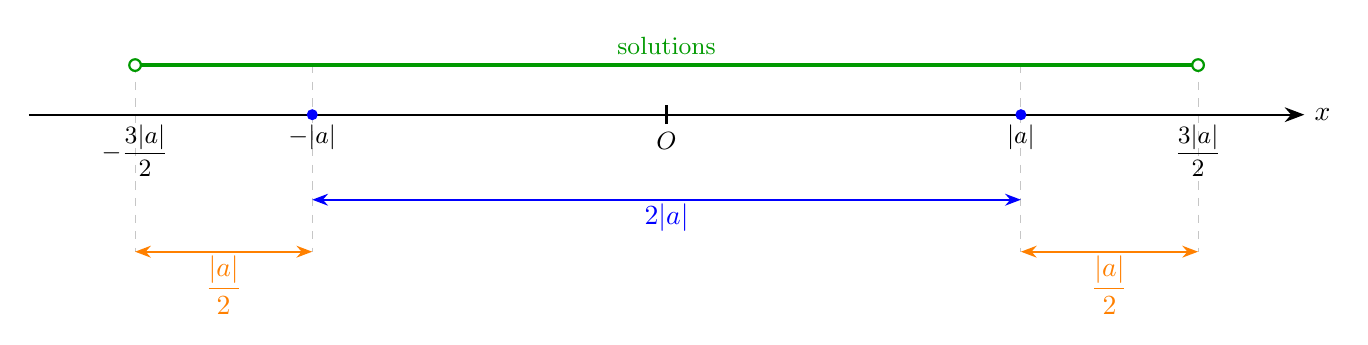
\begin{tikzpicture}[x=4.5cm,y=1.5cm]
\def\xmin{-1.8}
\def\xmax{1.8}
\def\leftend{-1.5}
\def\leftfixed{-1}
\def\rightfixed{1}
\def\rightend{1.5}
\def\soly{0.42}
\def\centraldim{-0.72}
\def\outerdim{-1.16}

% Vertical guides
\foreach \x in {\leftend,\leftfixed,\rightfixed,\rightend}{
  \draw[dashed, gray!45] (\x,\soly) -- (\x,\outerdim);
}

% Number line
\draw[thick, black, -{Stealth[length=2.5mm]}] (\xmin,0) -- (\xmax,0)
  node[right] {$x$};
\draw[thick] (0,-0.08) -- (0,0.08);

% Complete solution interval
\draw[very thick, green!60!black] (\leftend,\soly) -- (\rightend,\soly)
  node[midway, above] {\small solutions};
\foreach \x in {\leftend,\rightend}{
  \draw[thick, green!60!black, fill=white] (\x,\soly) circle[radius=2.1pt];
}

% Fixed points
\foreach \x in {\leftfixed,\rightfixed}{
  \fill[blue] (\x,0) circle[radius=2pt];
}

% Position labels
\node[below, font=\small] at (\leftend,0) {$-\dfrac{3|a|}{2}$};
\node[below, font=\small] at (\leftfixed,0) {$-|a|$};
\node[below=3pt, font=\small] at (0,0) {$O$};
\node[below, font=\small] at (\rightfixed,0) {$|a|$};
\node[below, font=\small] at (\rightend,0) {$\dfrac{3|a|}{2}$};

% Dimension arrows
\draw[blue, thick, {Stealth[length=2mm]}-{Stealth[length=2mm]}]
  (\leftfixed,\centraldim) -- (\rightfixed,\centraldim)
  node[midway, below, fill=white, inner sep=1pt] {$2|a|$};
\draw[orange, thick, {Stealth[length=2mm]}-{Stealth[length=2mm]}]
  (\leftend,\outerdim) -- (\leftfixed,\outerdim)
  node[midway, below, fill=white, inner sep=1pt] {$\dfrac{|a|}{2}$};
\draw[orange, thick, {Stealth[length=2mm]}-{Stealth[length=2mm]}]
  (\rightfixed,\outerdim) -- (\rightend,\outerdim)
  node[midway, below, fill=white, inner sep=1pt] {$\dfrac{|a|}{2}$};
\end{tikzpicture}
% end q000029 figure F1
\end{djsSolutionFigure}

If
\[
-|a|\leq x\leq |a|
\]
the two distances together equal the distance between the two fixed points, which is
\[
2|a|
\]
Hence every such $x$ satisfies the inequality because
\[
2|a|<3|a|
\]

Now suppose $x$ lies outside this central interval, at a distance $d$ from its nearer endpoint. Its distances from the two fixed points are then $d$ and $2|a|+d$, so their sum is
\[
2|a|+2d
\]
We require
\[
2|a|+2d<3|a|
\]
and hence
\[
d<\frac{|a|}{2}
\]

Thus there is an additional distance of $\dfrac{|a|}{2}$ available beyond each end of the central interval. The complete range is therefore
\[
-\frac{3|a|}{2}<x<\frac{3|a|}{2}
\]
The endpoints are excluded because they make the original left-hand side equal to $3|a|$, rather than less than $3|a|$

This is equivalent to
\[
|x|<\frac{3|a|}{2}
\]
Therefore the correct option is \textbf{C}.
% end q000029 solution
\end{djsSolution}
\end{enumerate}
\clearpage
\thispagestyle{djssolutions}
\vspace*{8pt}
\djsTopicLine{Differentiation}
\begin{enumerate}[label=\textbf{\arabic*.},leftmargin=*,itemsep=0pt,start=3]
\questionitem[Differentiation]
% begin q000624 stem
The diagram shows parts of the curves $y=x^2$ and $y=(x-2)^2+b$, where $b$ is positive. 

The curves meet at $P$, and the tangents to the curves at $P$ are perpendicular.

What is the value of $b$?
% end q000624 stem

\begin{center}
% begin q000624 diagram
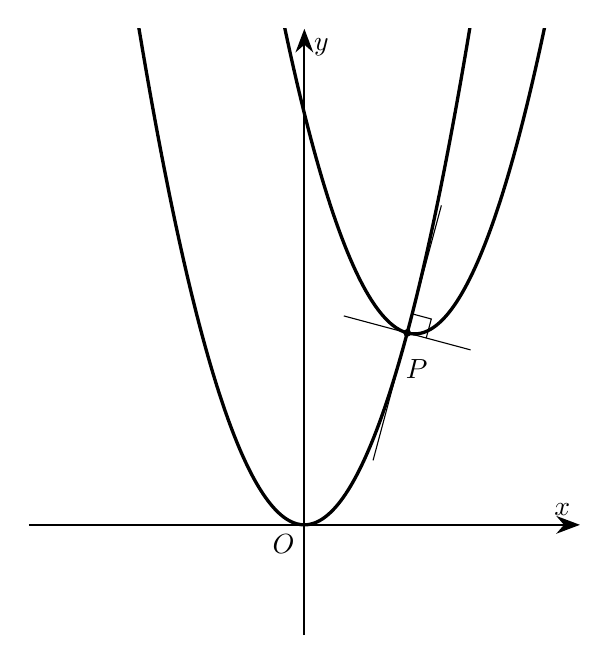
\begin{tikzpicture}
\pgfmathsetmacro{\px}{1+sqrt(3)/2}
\pgfmathsetmacro{\py}{\px*\px}
\pgfmathsetmacro{\bshift}{4*(\px-1)}
\pgfmathsetmacro{\mone}{2*\px}
\pgfmathsetmacro{\mtwo}{2*(\px-2)}
\pgfmathsetmacro{\tone}{0.62}
\pgfmathsetmacro{\ttwo}{1.15}
\pgfmathsetmacro{\tOnePX}{\px+\tone}
\pgfmathsetmacro{\tOnePY}{\py+\tone*\mone}
\pgfmathsetmacro{\tOneMX}{\px-\tone}
\pgfmathsetmacro{\tOneMY}{\py-\tone*\mone}
\pgfmathsetmacro{\tTwoPX}{\px+\ttwo}
\pgfmathsetmacro{\tTwoPY}{\py+\ttwo*\mtwo}
\pgfmathsetmacro{\tTwoMX}{\px-\ttwo}
\pgfmathsetmacro{\tTwoMY}{\py-\ttwo*\mtwo}
\begin{axis}[
    axis lines=middle,
    axis line style={thick,-{Stealth[length=3mm]}},
    xlabel={$x$},
    ylabel={$y$},
    xmin=-5, xmax=5,
    ymin=-2, ymax=9,
    xtick=\empty,
    ytick=\empty,
    width=7cm,
    height=12cm,
    scale only axis,
    axis equal image,
    enlargelimits=false,
    clip=true,
    samples=180
]
\addplot[very thick, black, domain=-4:3.2]
    {x^2}
    node[pos=0.12, above right] {$y=x^2$};
\addplot[very thick, black, domain=-1.2:5]
    {(x-2)^2+\bshift}
    node[pos=0.145, above right] {$y=(x-2)^2+b$};

\coordinate (P) at (axis cs:\px,\py);
\coordinate (TOnePlus) at (axis cs:\tOnePX,\tOnePY);
\coordinate (TOneMinus) at (axis cs:\tOneMX,\tOneMY);
\coordinate (TTwoPlus) at (axis cs:\tTwoPX,\tTwoPY);
\coordinate (TTwoMinus) at (axis cs:\tTwoMX,\tTwoMY);

\draw[thin, black] (TOneMinus) -- (TOnePlus);
\draw[thin, black] (TTwoMinus) -- (TTwoPlus);
\pic[draw, thin, angle radius=2.5mm]
    {right angle=TTwoPlus--P--TOnePlus};

\fill[black] (P) circle (1.4pt);
\node[anchor=south west, xshift=-4pt, yshift=-20pt] at (P) {$P$};
\node[below left] at (axis cs:0,0) {$O$};
\end{axis}
\end{tikzpicture}
% end q000624 diagram
\end{center}

\par\vspace*{12pt}
\begin{tabularx}{\linewidth}{@{}>{\bfseries}l Y@{}}
A &
% begin q000624 choice A
$\dfrac{\sqrt{3}}{2}$
% end q000624 choice A
\\[0.8em]
B &
% begin q000624 choice B
$\sqrt{3}$
% end q000624 choice B
\\[0.8em]
C &
% begin q000624 choice C
$2\sqrt{3}$
% end q000624 choice C
\\[0.8em]
D &
% begin q000624 choice D
$3\sqrt{3}$
% end q000624 choice D
\\[0.8em]
E &
% begin q000624 choice E
$4\sqrt{3}$
% end q000624 choice E
\\
\end{tabularx}

\begin{djsSolution}{C}
% begin q000624 solution
Let $x$ be the $x$-coordinate of $P$. Since $P$ lies on both curves, their $y$-coordinates are equal:
\[
x^2=(x-2)^2+b
\]
Expanding and rearranging gives
\[
b=4x-4=4(x-1)
\]
For the second curve, first write
\[
y=x^2-4x+4+b
\]
The gradients of the two curves at $P$ are therefore $2x$ and $2x-4$. 

Perpendicular lines have gradients that are negative reciprocals, so the product of their gradients is $-1$:
\[
(2x)(2x-4)=-1
\]
Hence
\[
4x^2-8x+1=0
\]
and the quadratic formula gives
\[
x=\frac{8\pm\sqrt{64-16}}{8}=1\pm\frac{\sqrt{3}}{2}
\]
For
\[
x=1+\frac{\sqrt{3}}{2},
\]
we obtain
\[
b=4(x-1)
=4\left(\frac{\sqrt{3}}{2}\right)
=2\sqrt{3}>0
\]

For
\[
x=1-\frac{\sqrt{3}}{2}
\]
we instead obtain
\[
b=4(x-1)
=4\left(-\frac{\sqrt{3}}{2}\right)
=-2\sqrt{3}<0
\]
which must be rejected since $b$ is positive.

Therefore
\[
b=2\sqrt{3}
\]
and the correct option is \textbf{C}.
% end q000624 solution
\end{djsSolution}
\end{enumerate}
\clearpage
\thispagestyle{djssolutions}
\vspace*{8pt}
\djsTopicLine{Algebra}
\begin{enumerate}[label=\textbf{\arabic*.},leftmargin=*,itemsep=0pt,start=4]
\questionitem[Algebra]
% begin q000586 stem
A positive real number $x$ satisfies
\[
(x-2)(x+3)(x+4)(x+9)=3024
\]
What is the value of $x^2+7x$?
% end q000586 stem

\par\vspace*{12pt}
\begin{tabularx}{\linewidth}{@{}>{\bfseries}l Y@{}}
A &
% begin q000586 choice A
$16$
% end q000586 choice A
\\[0.8em]
B &
% begin q000586 choice B
$38$
% end q000586 choice B
\\[0.8em]
C &
% begin q000586 choice C
$54$
% end q000586 choice C
\\[0.8em]
D &
% begin q000586 choice D
$60$
% end q000586 choice D
\\[0.8em]
E &
% begin q000586 choice E
$114$
% end q000586 choice E
\\
\end{tabularx}

\begin{djsSolution}{D}
% begin q000586 solution
Expanding all four factors would produce a quartic and create unnecessary work. Instead, notice that the two pairs $(x+3)(x+4)$ and $(x-2)(x+9)$ both have $7x$ as their linear term. Set
\[
A=x^2+7x
\]
Then
\[
(x+3)(x+4)=x^2+7x+12=A+12
\]
and
\[
(x-2)(x+9)=x^2+7x-18=A-18
\]
so the equation becomes
\[
(A-18)(A+12)=3024
\]
At this point, testing the options can be faster. For $A=60$,
\[
(A-18)(A+12)=42\times72=3024
\]
Thus the answer is option \textbf{D.}

For a complete algebraic solution, expanding gives
\[
A^2-6A-3240=0
\]
To factorise this, we need two numbers with product $-3240$ and sum $-6$. Since their sum is small, their magnitudes should be close. The prime factorisation helps to find them:
\[
3240=2^3\times3^4\times5=(2\times3^3)(2^2\times3\times5)=54\times60
\]
The required numbers are therefore $54$ and $-60$, giving
\[
(A-60)(A+54)=0
\]
Thus $A=60$ or $A=-54$. Since $x$ is positive, $A=x(x+7)>0$, so $A=-54$ is impossible. Hence $x^2+7x=60$, which is option \textbf{D}.

This question depends heavily on spotting the useful pairing of factors. If that pairing is not apparent quickly under exam conditions, it is sensible to skip the question and return later rather than expand a quartic.
% end q000586 solution
\end{djsSolution}
\end{enumerate}
\clearpage
\thispagestyle{djssolutions}
\vspace*{8pt}
\djsTopicLine{Integration}
\begin{enumerate}[label=\textbf{\arabic*.},leftmargin=*,itemsep=0pt,start=5]
\questionitem[Integration]
% begin q000603 stem
The curve $y = x^3 - 3x + 5$ has a tangent line at the point where $x = 2$. 

This tangent meets the curve again at exactly one other point. Find the area of the region enclosed between the curve and the tangent.
% end q000603 stem

\par\vspace*{12pt}
\begin{tabularx}{\linewidth}{@{}>{\bfseries}l Y@{}}
A &
% begin q000603 choice A
$-108$
% end q000603 choice A
\\[0.8em]
B &
% begin q000603 choice B
$54$
% end q000603 choice B
\\[0.8em]
C &
% begin q000603 choice C
$96$
% end q000603 choice C
\\[0.8em]
D &
% begin q000603 choice D
$108$
% end q000603 choice D
\\[0.8em]
E &
% begin q000603 choice E
$120$
% end q000603 choice E
\\[0.8em]
F &
% begin q000603 choice F
$216$
% end q000603 choice F
\\
\end{tabularx}

\begin{djsSolution}{D}
% begin q000603 solution
Differentiate the equation of the curve:
\[
\frac{\mathrm{d}y}{\mathrm{d}x}=3x^2-3
\]
At $x=2$, the gradient is $3(2^2)-3=9$, and the point on the curve is $(2,7)$. Hence the tangent has equation
\[
y-7=9(x-2)
\]
so
\[
y=9x-11
\]
To find the other intersection, equate the curve and tangent:
\[
x^3-3x+5=9x-11
\]
Therefore
\[
x^3-12x+16=0
\]

Since the tangent touches the curve at $x=2$, the factor $(x-2)$ of this cubic occurs twice as $(x-2)^2$. The other factor must therefore be $(x+4)$ to make the leading term of $x^3$ and the constant term of $16$.

Hence, or otherwise, this cubic factorises as
\[
x^3-12x+16=(x-2)^2(x+4)
\]
Thus the other intersection is at $x=-4$.

The area between curves $y=f(x)$ and $y=g(x)$ from $x=a$ to $x=b$, when $f(x)\geq g(x)$, is
\[
A=\int_a^b \bigl(f(x)-g(x)\bigr)\,\mathrm{d}x
\]

Here, one can check that the curve lies above the tangent for $-4\leq x\leq2$ so this formula is appropriate. Hence
\[
\begin{aligned}
A &=\int_{-4}^{2}(x^3-3x+5)-(9x-11)\,\mathrm{d}x\\
&=\int_{-4}^{2}(x^3-12x+16)\,\mathrm{d}x\\
&=\left[\frac{x^4}{4}-6x^2+16x\right]_{-4}^{2} =12-(-96) =108
\end{aligned}
\]
Therefore the correct option is \textbf{D}.
% end q000603 solution
\end{djsSolution}
\end{enumerate}
\clearpage
\thispagestyle{djssolutions}
\vspace*{8pt}
\djsTopicLine{Coordinate Geometry}
\begin{enumerate}[label=\textbf{\arabic*.},leftmargin=*,itemsep=0pt,start=6]
\questionitem[Coordinate Geometry]
% begin q000633 stem
A straight line passes through the point $(2, 5)$ and has gradient $m$.

The line forms a triangle of area $25$ with the positive $x$-axis and the positive $y$-axis.

What is the sum of all possible values of $m$?
% end q000633 stem

\par\vspace*{12pt}
\begin{tabularx}{\linewidth}{@{}>{\bfseries}l Y@{}}
A &
% begin q000633 choice A
$-15$
% end q000633 choice A
\\[0.8em]
B &
% begin q000633 choice B
$-\dfrac{15}{2}$
% end q000633 choice B
\\[0.8em]
C &
% begin q000633 choice C
$-\dfrac{25}{4}$
% end q000633 choice C
\\[0.8em]
D &
% begin q000633 choice D
$-\dfrac{15}{4}$
% end q000633 choice D
\\[0.8em]
E &
% begin q000633 choice E
$\dfrac{15}{2}$
% end q000633 choice E
\\
\end{tabularx}

\begin{djsSolution}{B}
% begin q000633 solution
The geometry is represented by the following sketch.

\begin{djsSolutionFigure}
% begin q000633 figure F1
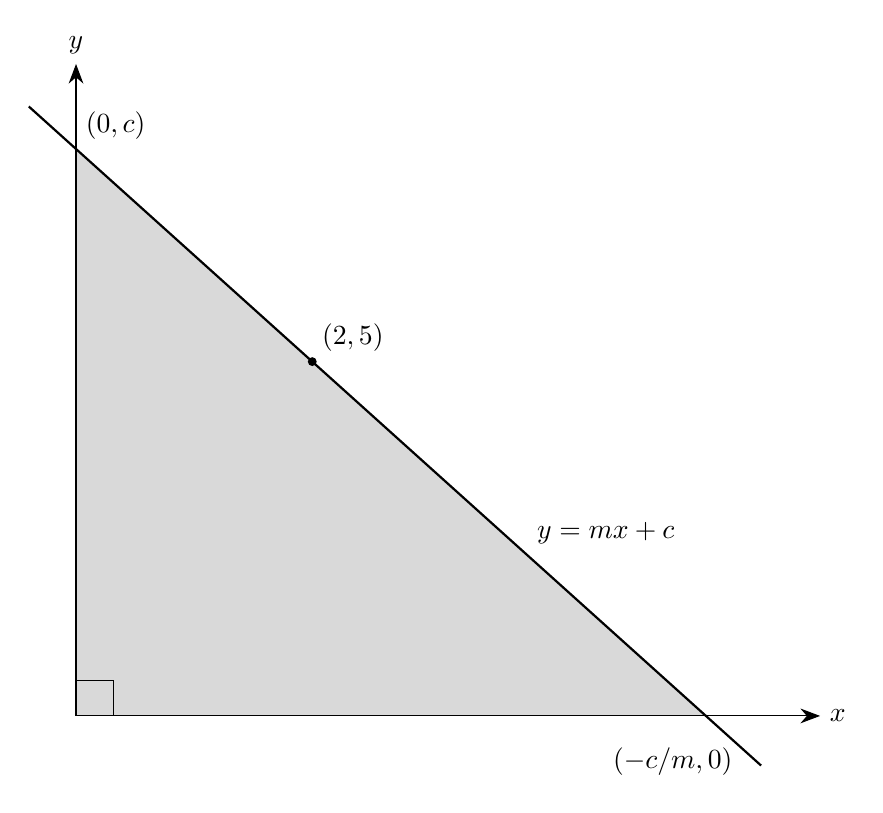
\begin{tikzpicture}[x=1.5cm,y=0.90cm]
\coordinate (O) at (0,0);
\coordinate (B) at (0,8);
\coordinate (P) at (2,5);
\coordinate (A) at ({16/3},0);
\coordinate (L) at (-0.4,8.6);
\coordinate (R) at (5.8,-0.7);

\fill[gray!30] (O) -- (A) -- (B) -- cycle;

\draw[-{Stealth[length=2.5mm]},black] (O) -- (6.3,0)
    node[right] {$x$};
\draw[-{Stealth[length=2.5mm]},black] (O) -- (0,9.2)
    node[above] {$y$};

\draw[thick,black] (L) -- (R)
    node[pos=0.68,above right] {$y=mx+c$};

\fill[black] (P) circle (1.6pt);
\node[above right] at (P) {$(2,5)$};
\node[above right] at (B) {$(0,c)$};
\node[below, yshift=-8pt, xshift=-12pt] at (A) {$(-c/m,0)$};

\draw[black] (0,0.5) -- (0.32,0.5) -- (0.32,0);
\end{tikzpicture}
% end q000633 figure F1
\end{djsSolutionFigure}

The two intercepts must both lie on the positive axes, so the line slopes downwards from left to right. Hence $m<0$.

Write the equation of the line as
\[
y=mx+c
\]
Since it passes through $(2,5)$,
\[
5=2m+c
\]
so its $y$-intercept is
\[
c=5-2m
\]
At the $x$-intercept, $y=0$, so
\[
0=mx+c
\]
and therefore the $x$-intercept is $-\dfrac{c}{m}$. This is positive because $c>0$ and $m<0$.

The triangle consequently has base $-\dfrac{c}{m}$ and height $c$. Using its area gives
\[
25=\frac12\left(-\frac{c}{m}\right)c=-\frac{c^2}{2m}
\]
Substituting $c=5-2m$ and multiplying by $2m$, which is non-zero, gives
\[
(5-2m)^2=-50m
\]
Therefore
\[
4m^2+30m+25=0
\]
The quadratic formula gives
\[
m=\frac{-30\pm\sqrt{30^2-4\times4\times25}}{8}
 =\frac{-15\pm5\sqrt5}{4}
\]
Both values are negative and hence both give positive intercepts, so both are valid. Their sum is
\[
\frac{-15+5\sqrt5}{4}+\frac{-15-5\sqrt5}{4}
=-\frac{15}{2}
\]

As a shortcut, for $Ax^2+Bx+C=0$, the sum of the roots is $-\dfrac{B}{A}$ and their product is $\dfrac{C}{A}$.

Thus the sum could have been read directly from $4m^2+30m+25=0$ as $-\dfrac{30}{4}=-\dfrac{15}{2}$.

Therefore the correct option is \textbf{B}.
% end q000633 solution
\end{djsSolution}
\end{enumerate}
\clearpage
\thispagestyle{djssolutions}
\vspace*{8pt}
\djsTopicLine{Number}
\begin{enumerate}[label=\textbf{\arabic*.},leftmargin=*,itemsep=0pt,start=7]
\questionitem[Number]
% begin q000641 stem
Consider the integer
\[N = 8^{15}\times 5^{40}\]
When $N$ is written out in full, how many digits does it have?
% end q000641 stem

\par\vspace*{12pt}
\begin{tabularx}{\linewidth}{@{}>{\bfseries}l Y@{}}
A &
% begin q000641 choice A
$40$
% end q000641 choice A
\\[0.8em]
B &
% begin q000641 choice B
$41$
% end q000641 choice B
\\[0.8em]
C &
% begin q000641 choice C
$42$
% end q000641 choice C
\\[0.8em]
D &
% begin q000641 choice D
$43$
% end q000641 choice D
\\[0.8em]
E &
% begin q000641 choice E
$46$
% end q000641 choice E
\\[0.8em]
F &
% begin q000641 choice F
$55$
% end q000641 choice F
\\
\end{tabularx}

\begin{djsSolution}{C}
% begin q000641 solution
Calculating $N$ in full is inefficient. Instead, pair factors of $2$ and $5$ to produce powers of $10$.

Since $8^{15}=2^{45}$,
\[
N=2^{45}\times 5^{40}=2^5\times (2\times 5)^{40}=32\times 10^{40}=3.2\times 10^{41}
\]
Thus $10^{41}\leq N<10^{42}$, so $N$ has $42$ digits. 

Equivalently, $32\times10^{40}$ is $32$ followed by $40$ zeros, giving $2+40=42$ digits.

Therefore the correct option is \textbf{C}.
% end q000641 solution
\end{djsSolution}
\end{enumerate}
\clearpage
\thispagestyle{djssolutions}
\vspace*{8pt}
\djsTopicLine{Sequences \& Series}
\begin{enumerate}[label=\textbf{\arabic*.},leftmargin=*,itemsep=0pt,start=8]
\questionitem[Sequences \& Series]
% begin q000650 stem
The $n$th term of a sequence is a quadratic expression in $n$. 

The second, fifth and eighth terms are $4$, $13$ and $40$, respectively. 

What is the eleventh term?
% end q000650 stem

\par\vspace*{12pt}
\begin{tabularx}{\linewidth}{@{}>{\bfseries}l Y@{}}
A &
% begin q000650 choice A
$67$
% end q000650 choice A
\\[0.8em]
B &
% begin q000650 choice B
$76$
% end q000650 choice B
\\[0.8em]
C &
% begin q000650 choice C
$85$
% end q000650 choice C
\\[0.8em]
D &
% begin q000650 choice D
$94$
% end q000650 choice D
\\[0.8em]
E &
% begin q000650 choice E
$121$
% end q000650 choice E
\\
\end{tabularx}

\begin{djsSolution}{C}
% begin q000650 solution
Write the $n$th term as
\[
an^2+bn+c
\]
Using the three given terms gives
\[
\begin{aligned}
4a+2b+c&=4 \\
25a+5b+c&=13 \\
64a+8b+c&=40
\end{aligned}
\]
Subtracting the first equation from the second, and the second from the third, eliminates $c$:
\[
\begin{aligned}
21a+3b&=9 \\
39a+3b&=27
\end{aligned}
\]
Subtracting these equations gives $18a=18$, so $a=1$. Hence $21+3b=9$, giving $b=-4$. Substitution into the first original equation then gives
\[
4-8+c=4
\]
so $c=8$. Therefore the $n$th term is 
\[n^2-4n+8\]
so, in particular, the 11th term is
\[
11^2-4(11)+8=121-44+8=85
\]
Thus the correct option is \textbf{C}. \\[5pt]

\textit{Alternative Solution:}

From GCSE, we know that a quadratic sequence has constant second differences.

Taking terms at equally spaced positions preserves this property: if we take every third term of a quadratic sequence, the resulting sequence is still quadratic, so its second differences are still constant. (In fact, taking every third term multiplies the second difference by \(3^2=9\))

Here the positions \((2,\,5,\,8,\,11,\,\ldots)\) are equally spaced, so we can work directly with the given terms as a quadratic sequence.

The differences between the known terms are
\[
13-4=9,\qquad 40-13=27
\]
so the second difference is $27-9=18$. The next first difference must therefore be
\[
27+18=45
\]
Hence the next term is $40+45=85$, so the correct option is again \textbf{C}.
% end q000650 solution
\end{djsSolution}
\end{enumerate}
\clearpage
\thispagestyle{djssolutions}
\vspace*{8pt}
\djsTopicLine{Geometry}
\begin{enumerate}[label=\textbf{\arabic*.},leftmargin=*,itemsep=0pt,start=9]
\questionitem[Geometry]
% begin q000635 stem
A circle of radius $1$ lies in the region where $x\ge 0$ and $y\ge 0$, and touches both axes.

A second, smaller circle also lies in this region, touches both axes, and touches the first circle at exactly one point. 

The two circles do not overlap.

What is the radius of the smaller circle?
% end q000635 stem

\begin{center}
% begin q000635 diagram
\begin{tikzpicture}[scale=2.5]
\def\R{1}
\def\xmax{2.6}
\def\ymax{2.6}
\pgfmathsetmacro{\rsmall}{\R*(sqrt(2)-1)/(sqrt(2)+1)}

\coordinate (O) at (0,0);
\coordinate (C) at (\R,\R);
\coordinate (D) at (\rsmall,\rsmall);
\coordinate (B) at (\R,0);
\coordinate (T) at ($(D)+(45:\rsmall)$);

\draw[-{Stealth[length=3mm]}] (O) -- (\xmax,0) node[right] {$x$};
\draw[-{Stealth[length=3mm]}] (O) -- (0,\ymax) node[above] {$y$};

\draw[thick, black] (C) circle (\R);
\draw[thick, black] (D) circle (\rsmall);

\end{tikzpicture}
% end q000635 diagram
\end{center}

\par\vspace*{12pt}
\begin{tabularx}{\linewidth}{@{}>{\bfseries}l Y@{}}
A &
% begin q000635 choice A
$\dfrac{1}{3}$
% end q000635 choice A
\\[0.8em]
B &
% begin q000635 choice B
$3-2\sqrt{2}$
% end q000635 choice B
\\[0.8em]
C &
% begin q000635 choice C
$\sqrt{2}-1$
% end q000635 choice C
\\[0.8em]
D &
% begin q000635 choice D
$\dfrac{\sqrt{2}-1}{2}$
% end q000635 choice D
\\[0.8em]
E &
% begin q000635 choice E
$2-\sqrt{2}$
% end q000635 choice E
\\[0.8em]
F &
% begin q000635 choice F
$17-12\sqrt{2}$
% end q000635 choice F
\\[0.8em]
G &
% begin q000635 choice G
$3+2\sqrt{2}$
% end q000635 choice G
\\
\end{tabularx}

\begin{djsSolution}{B}
% begin q000635 solution
Let the smaller radius be $r$. A circle tangent to both axes has its centre one radius from each axis. Therefore the centres of the large and small circles are respectively $C=(1,1)$ and $D=(r,r)$.

The horizontal and vertical distances between the centres are both $1-r$. Also, because the circles touch externally without overlapping, the distance between their centres is the sum of their radii, $1+r$.

\begin{djsSolutionFigure}
% begin q000635 figure F1
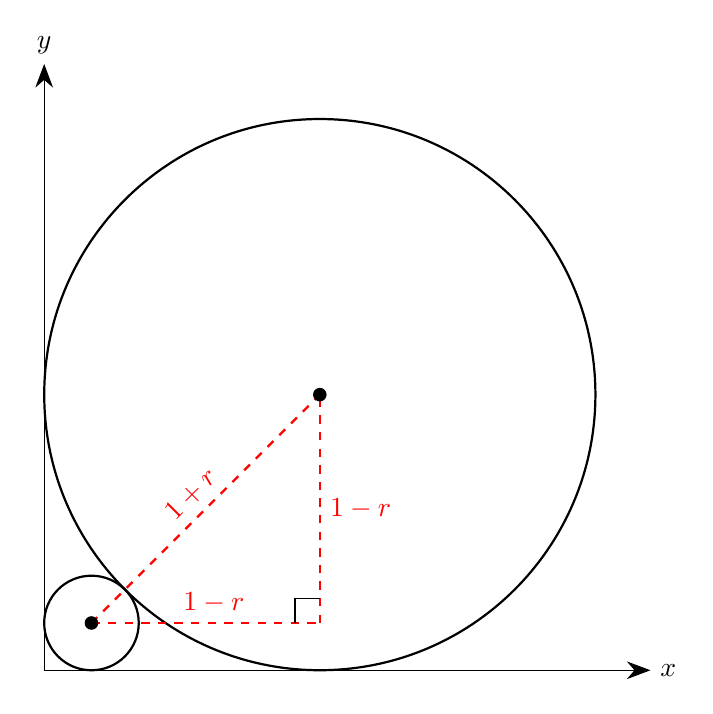
\begin{tikzpicture}[scale=3.5]
\def\R{1}
\def\xmax{2.2}
\def\ymax{2.2}
\pgfmathsetmacro{\rsmall}{\R*(sqrt(2)-1)/(sqrt(2)+1)}

\coordinate (O) at (0,0);
\coordinate (C) at (\R,\R);
\coordinate (D) at (\rsmall,\rsmall);
\coordinate (B) at (\R,0);
\coordinate (T) at ($(D)+(45:\rsmall)$);

\draw[-{Stealth[length=3mm]}] (O) -- (\xmax,0) node[right] {$x$};
\draw[-{Stealth[length=3mm]}] (O) -- (0,\ymax) node[above] {$y$};

\draw[thick, black] (C) circle (\R);
\draw[thick, black] (D) circle (\rsmall);

\coordinate (P) at (\R,\rsmall);
\def\ramark{0.09}

\draw[thick, dashed, red] (D) -- node[above, sloped] {$1+r$} (C);
\draw[thick, dashed, red] (D) -- node[above, xshift=3pt] {$1-r$} (P);
\draw[thick, dashed, red] (P) -- node[right] {$1-r$} (C);

\draw[thin, black]
  ($(P)+(-\ramark,0)$) --
  ($(P)+(-\ramark,\ramark)$) --
  ($(P)+(0,\ramark)$);

\fill (C) circle (0.7pt);
\fill (D) circle (0.7pt);

\end{tikzpicture}
% end q000635 figure F1
\end{djsSolutionFigure}

The line joining the centres is therefore the hypotenuse of a right-angled triangle whose other two sides both have length $1-r$. Pythagoras' theorem gives
\[
(1+r)^2=(1-r)^2+(1-r)^2
\]
Expanding and rearranging gives
\[
1+2r+r^2=2-4r+2r^2
\]
\[
r^2-6r+1=0
\]
Using the quadratic formula,
\[
r=\frac{6\pm\sqrt{36-4}}{2}=3\pm2\sqrt{2}
\]
The smaller circle must have $0<r<1$. The root $3+2\sqrt{2}$ is greater than $1$, so it is rejected. Also, $2\sqrt{2}<3$ and $2\sqrt{2}>2$, so $0<3-2\sqrt{2}<1$.

Therefore the radius is $3-2\sqrt{2}$, which is option \textbf{B}.
% end q000635 solution
\end{djsSolution}
\end{enumerate}
\clearpage
\thispagestyle{djssolutions}
\vspace*{8pt}
\djsTopicLine{Sequences \& Series}
\begin{enumerate}[label=\textbf{\arabic*.},leftmargin=*,itemsep=0pt,start=10]
\questionitem[Sequences \& Series]
% begin q000048 stem
A sequence $a_n$ is defined by $a_0=3$ and, for $n\ge 0$, \[ a_{n+1}=3(a_n)^2 \] Which of the following is equal to $\log_3(a_n)$?
% end q000048 stem

\par\vspace*{12pt}
\begin{tabularx}{\linewidth}{@{}>{\bfseries}l Y@{}}
A &
% begin q000048 choice A
$2^n$
% end q000048 choice A
\\[0.8em]
B &
% begin q000048 choice B
$2^n-1$
% end q000048 choice B
\\[0.8em]
C &
% begin q000048 choice C
$2^{n+1}-1$
% end q000048 choice C
\\[0.8em]
D &
% begin q000048 choice D
$2^{n+1}+1$
% end q000048 choice D
\\[0.8em]
E &
% begin q000048 choice E
$2^{n}-2$
% end q000048 choice E
\\[0.8em]
F &
% begin q000048 choice F
$2^{n+1}-2$
% end q000048 choice F
\\
\end{tabularx}

\begin{djsSolution}{C}
% begin q000048 solution
Trying the options is exceptionally effective here. Since $a_0=3$,
\[
\log_3(a_0)=1
\]
At $n=0$, option A gives $2^0=1$ and option C gives $2^1-1=1$. Every other option gives a value different from $1$, so only A and C remain.

Now
\[
a_1=3(3)^2=27
\]
Therefore $\log_3(a_1)=3$. At $n=1$, option A gives $2$, whereas option C gives $2^2-1=3$. Hence the correct option is \textbf{C}.\\[5pt]

\textit{Alternative Solution:} 

Now lets actually solve the problem by finding the $n$th term. Let
\[
b_n=\log_3(a_n)
\]
Taking logarithms of the recurrence gives
\begin{align*}
    b_{n+1}&=\log_3a_{n+1}\\
           &=\log_3\bigl(3(a_n)^2\bigr)\\
           &= 1 + 2\log_3a_n \\
           &=1+2b_n
\end{align*}
This recurrence contains both multiplication and addition. The sequence is therefore neither arithmetic or geometric, but a mixture of the two.

However, we can turn it into a geometric sequence. Adding $1$ to both sides:
\[
b_{n+1}+1=2(b_n+1)
\]
Define $c_n=b_n+1$. Then
\[
c_{n+1}=2c_n
\]

So $c_n$ is a geometric sequence with common ratio $2$. Also, $b_0=\log_3 3=1$, so $c_0=2$. Thus the first term of the geometric sequence is $2$.

The usual geometric sequence formula for the $n$th term is $ar^{n-1}$ for the term in position $n$. Here $c_n$ is in position $n+1$ because the indexing begins at $n=0$. 

Therefore
\begin{align*}
    c_n&=ar^{(n+1)-1} \\
    &=2\cdot 2^{(n+1)-1}\\
    &=2^{n+1}
\end{align*}
Since $b_n=c_n-1$,
\[
\log_3(a_n)=b_n=2^{n+1}-1
\]
Which again obtains option \textbf{C}.

The full recurrence method is instructive but far more involved, making this a good example of when trying the options first is the right exam technique.
% end q000048 solution
\end{djsSolution}
\end{enumerate}
\clearpage
\thispagestyle{djssolutions}
\vspace*{8pt}
\djsTopicLine{Number}
\begin{enumerate}[label=\textbf{\arabic*.},leftmargin=*,itemsep=0pt,start=11]
\questionitem[Number]
% begin q000567 stem
An integer $n$ is chosen at random from the integers $1$ to $1260$ inclusive, with each integer equally likely to be chosen. 

The fraction $\dfrac{n}{1260}$ is written as a decimal.

What is the probability that this decimal terminates and that its shortest form has exactly two digits after the decimal point?

In the shortest form, zeros at the end are omitted; for example, $0.50$ is written as $0.5$.
% end q000567 stem

\par\vspace*{12pt}
\begin{tabularx}{\linewidth}{@{}>{\bfseries}l Y@{}}
A &
% begin q000567 choice A
$\dfrac{1}{630}$
% end q000567 choice A
\\[0.8em]
B &
% begin q000567 choice B
$\dfrac{2}{315}$
% end q000567 choice B
\\[0.8em]
C &
% begin q000567 choice C
$\dfrac{1}{126}$
% end q000567 choice C
\\[0.8em]
D &
% begin q000567 choice D
$\dfrac{1}{90}$
% end q000567 choice D
\\[0.8em]
E &
% begin q000567 choice E
$\dfrac{1}{70}$
% end q000567 choice E
\\[0.8em]
F &
% begin q000567 choice F
$\dfrac{1}{63}$
% end q000567 choice F
\\
\end{tabularx}

\begin{djsSolution}{C}
% begin q000567 solution
A fraction in its lowest terms has a terminating decimal if and only if its denominator has no prime factors other than $2$ and $5$.

Indeed, a terminating decimal with $r$ decimal places can be written with denominator $10^r=2^r5^r$, so its reduced denominator can contain only these two prime factors. Conversely, if the denominator is $2^a5^b$, multiplying the numerator and denominator by suitable powers of $2$ and $5$ produces a denominator that is a power of $10$. For example,
\[
\frac{3}{8}=\frac{375}{1000}=0.375
\]
By contrast, the factor $3$ in the reduced denominator of $\frac16$ cannot be removed in this way, and its decimal does not terminate.

Similarly, a terminating decimal has at most two digits after the decimal point if and only if its reduced denominator divides $100$. It has at most one digit if and only if its reduced denominator divides $10$. Therefore, it has exactly two digits in its shortest form if its reduced denominator divides $100$ but does not divide $10$. For example, $\frac{3}{20}=0.15$ has two digits, whereas $\frac12=0.5$ has only one.

Factorising the original denominator gives
\[
1260=2^2\times 3^2\times 5\times 7
\]
Any reduced denominator must divide $1260$. The divisors of both $1260$ and $100$ are the divisors of $20$, namely
\[
1,2,4,5,10,20
\]
Removing those that divide $10$ leaves reduced denominators $4$ and $20$.

For reduced denominator $4$, write
\[
\frac{n}{1260}=\frac{a}{4}
\]
Then $n=315a$. The allowed numerators are $a=1,3$, giving $2$ possible values of $n$.

For reduced denominator $20$, $n=63a$. The integers from $1$ to $20$ having no factor $2$ or $5$ in common with $20$ are
\[
1,3,7,9,11,13,17,19
\]
This gives another $8$ possible values of $n$. Hence there are $10$ successful choices out of $1260$, so the required probability is
\[
\frac{10}{1260}=\frac{1}{126}
\]
Therefore the correct option is \textbf{C}.
% end q000567 solution
\end{djsSolution}
\end{enumerate}
\clearpage
\thispagestyle{djssolutions}
\vspace*{8pt}
\djsTopicLine{Functions \& Graphs}
\begin{enumerate}[label=\textbf{\arabic*.},leftmargin=*,itemsep=0pt,start=12]
\questionitem[Functions \& Graphs]
% begin q000573 stem
A function $f$ has the form $f(x)=ax+b$, where $a$ and $b$ are real constants.

For every real $x$, applying $f$ twice gives
\[
f(f(x))=4x+3
\]

What is the difference between the greatest and least possible values of $f(2)$?
% end q000573 stem

\par\vspace*{12pt}
\begin{tabularx}{\linewidth}{@{}>{\bfseries}l Y@{}}
A &
% begin q000573 choice A
$2$
% end q000573 choice A
\\[0.8em]
B &
% begin q000573 choice B
$4$
% end q000573 choice B
\\[0.8em]
C &
% begin q000573 choice C
$7$
% end q000573 choice C
\\[0.8em]
D &
% begin q000573 choice D
$10$
% end q000573 choice D
\\[0.8em]
E &
% begin q000573 choice E
$12$
% end q000573 choice E
\\[0.8em]
F &
% begin q000573 choice F
$14$
% end q000573 choice F
\\
\end{tabularx}

\begin{djsSolution}{E}
% begin q000573 solution
Composing the function with itself gives
\[
f(f(x))=a(ax+b)+b=a^2x+b(a+1)
\]
Since this equals $4x+3$ for every real $x$, the corresponding coefficients must be equal. Hence
\[
a^2=4 \quad\text{and}\quad b(a+1)=3
\]
Since \(a^2=4\) there are two possible values of $a$, $a=2$ or $a=-2$

If $a=2$, then $3b=3$, so $b=1$ and
\[
f(2)=2(2)+1=5
\]
If $a=-2$, then $-b=3$, so $b=-3$ and
\[
f(2)=-2(2)-3=-7
\]
The greatest possible value is $5$ and the least is $-7$, so their difference is
\[
5-(-7)=12
\]
Therefore the correct option is \textbf{E}.
% end q000573 solution
\end{djsSolution}
\end{enumerate}
\clearpage
\thispagestyle{djssolutions}
\vspace*{8pt}
\djsTopicLine{Algebra}
\begin{enumerate}[label=\textbf{\arabic*.},leftmargin=*,itemsep=0pt,start=13]
\questionitem[Algebra]
% begin q000595 stem
The equation $x^2-7x+1=0$ has two positive solutions, $p$ and $q$.

What is the value of

\[ \frac{p-1}{p+1}\times\frac{q-1}{q+1} \,\, \mathrm{?}\]
% end q000595 stem

\par\vspace*{12pt}
\begin{tabularx}{\linewidth}{@{}>{\bfseries}l Y@{}}
A &
% begin q000595 choice A
$-\dfrac{2}{3}$
% end q000595 choice A
\\[0.8em]
B &
% begin q000595 choice B
$-\dfrac{5}{8}$
% end q000595 choice B
\\[0.8em]
C &
% begin q000595 choice C
$-\dfrac{5}{9}$
% end q000595 choice C
\\[0.8em]
D &
% begin q000595 choice D
$\dfrac{5}{9}$
% end q000595 choice D
\\[0.8em]
E &
% begin q000595 choice E
$\dfrac{5}{8}$
% end q000595 choice E
\\[0.8em]
F &
% begin q000595 choice F
$\dfrac{2}{3}$
% end q000595 choice F
\\
\end{tabularx}

\begin{djsSolution}{C}
% begin q000595 solution
For a quadratic $ax^2+bx+c=0$, the sum of the roots is $-b/a$ and their product is $c/a$. Therefore
\[
p+q=7 \qquad\text{and}\qquad pq=1
\]
Combine the two fractions before substituting these values:

\[
\frac{p-1}{p+1}\times\frac{q-1}{q+1}
=\frac{(p-1)(q-1)}{(p+1)(q+1)}
=\frac{pq-(p+q)+1}{pq+(p+q)+1}
\]

Hence the required value is

\[
\frac{1-7+1}{1+7+1}=-\frac{5}{9}
\]

Thus the correct option is \textbf{C}. \\[5pt]

\textit{Alternative Solution:}

The quadratic formula gives
\[
p=\frac{7+3\sqrt5}{2} \qquad\text{and}\qquad q=\frac{7-3\sqrt5}{2}
\]

Substitution and rationalising then gives

\[
\frac{p-1}{p+1}\times\frac{q-1}{q+1}
=\frac{5+3\sqrt5}{9+3\sqrt5}\times\frac{5-3\sqrt5}{9-3\sqrt5}
=\frac{25-45}{81-45}
=-\frac{5}{9}
\]

Again obtaining option \textbf{C}.

This route works, but the surd manipulation is longer and may waste time; using the sum and product of the roots is much more efficient.
% end q000595 solution
\end{djsSolution}
\end{enumerate}
\clearpage
\thispagestyle{djssolutions}
\vspace*{8pt}
\djsTopicLine{Probability \& Counting}
\begin{enumerate}[label=\textbf{\arabic*.},leftmargin=*,itemsep=0pt,start=14]
\questionitem[Probability \& Counting]
% begin q000658 stem
A cube has edge length $1$. 

Three different vertices are chosen at random. 

Every choice of three vertices is equally likely.

What is the probability that the three chosen vertices form a right-angled triangle?
% end q000658 stem

\begin{center}
% begin q000658 diagram
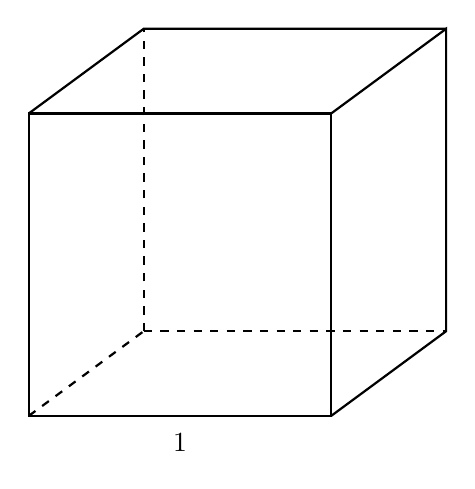
\begin{tikzpicture}[
    scale=1.2,
    x={(1cm,0cm)},
    y={(0.38cm,0.28cm)},
    z={(0cm,1cm)}
]
\def\side{3.2}

\coordinate (FBL) at (0,0,0);
\coordinate (FBR) at (\side,0,0);
\coordinate (FTR) at (\side,0,\side);
\coordinate (FTL) at (0,0,\side);
\coordinate (RBL) at (0,\side,0);
\coordinate (RBR) at (\side,\side,0);
\coordinate (RTR) at (\side,\side,\side);
\coordinate (RTL) at (0,\side,\side);

% Hidden edges
\draw[thick, black, dashed] (FBL) -- (RBL);
\draw[thick, black, dashed] (RBL) -- (RBR);
\draw[thick, black, dashed] (RBL) -- (RTL);

% Visible edges
\draw[thick, black] (FBL) -- (FBR) -- (FTR) -- (FTL) -- cycle;
\draw[thick, black] (FBR) -- (RBR) -- (RTR) -- (FTR);
\draw[thick, black] (FTL) -- (RTL) -- (RTR);

\node[below=3pt] at ($(FBL)!0.5!(FBR)$) {$1$};
\end{tikzpicture}
% end q000658 diagram
\end{center}

\par\vspace*{12pt}
\begin{tabularx}{\linewidth}{@{}>{\bfseries}l Y@{}}
A &
% begin q000658 choice A
$\dfrac{3}{7}$
% end q000658 choice A
\\[0.8em]
B &
% begin q000658 choice B
$\dfrac{1}{2}$
% end q000658 choice B
\\[0.8em]
C &
% begin q000658 choice C
$\dfrac{4}{7}$
% end q000658 choice C
\\[0.8em]
D &
% begin q000658 choice D
$\dfrac{3}{4}$
% end q000658 choice D
\\[0.8em]
E &
% begin q000658 choice E
$\dfrac{6}{7}$
% end q000658 choice E
\\[0.8em]
F &
% begin q000658 choice F
$1$
% end q000658 choice F
\\
\end{tabularx}

\begin{djsSolution}{E}
% begin q000658 solution
The distance between two cube vertices is one of $1$, $\sqrt2$ and $\sqrt3$, according as they are joined by an edge, a face diagonal or a space diagonal.

Any triangle containing a space diagonal has side lengths $1,\sqrt2,\sqrt3$, so it is right-angled since
\[
1^2+(\sqrt2)^2=(\sqrt3)^2.
\]
If there is no space diagonal but the triangle contains an edge, its side lengths are $1,1,\sqrt2$, so it is again right-angled.

Hence the only non-right-angled triangles have all three sides equal to $\sqrt2$: they are formed entirely from face diagonals.

Fix the upper and lower faces of the cube. For any vertex $A$, there are exactly two vertices on the opposite horizontal face that are a face diagonal away from $A$, and these two vertices are themselves a face diagonal apart. Thus they form the equilateral triangle shown below.

\begin{djsSolutionFigure}
% begin q000658 figure F1
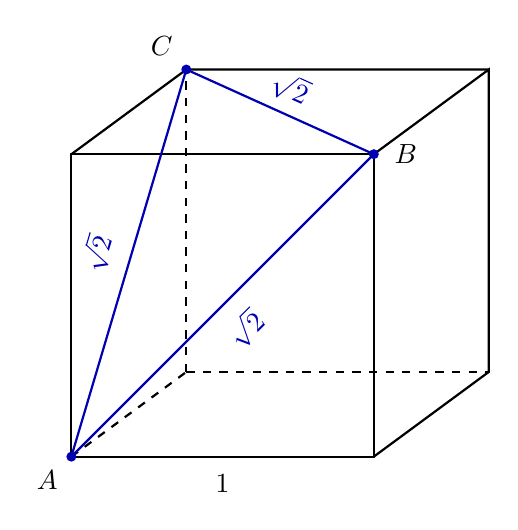
\begin{tikzpicture}[
    scale=1.2,
    x={(1cm,0cm)},
    y={(0.38cm,0.28cm)},
    z={(0cm,1cm)}
]
\def\side{3.2}

\coordinate (FBL) at (0,0,0);
\coordinate (FBR) at (\side,0,0);
\coordinate (FTR) at (\side,0,\side);
\coordinate (FTL) at (0,0,\side);
\coordinate (RBL) at (0,\side,0);
\coordinate (RBR) at (\side,\side,0);
\coordinate (RTR) at (\side,\side,\side);
\coordinate (RTL) at (0,\side,\side);

% Hidden edges
\draw[thick, black, dashed] (FBL) -- (RBL);
\draw[thick, black, dashed] (RBL) -- (RBR);
\draw[thick, black, dashed] (RBL) -- (RTL);

% Visible edges
\draw[thick, black] (FBL) -- (FBR) -- (FTR) -- (FTL) -- cycle;
\draw[thick, black] (FBR) -- (RBR) -- (RTR) -- (FTR);
\draw[thick, black] (FTL) -- (RTL) -- (RTR);

\node[below=3pt] at ($(FBL)!0.5!(FBR)$) {$1$};

% Equilateral triangle formed by three face diagonals
\coordinate (A) at (FBL);
\coordinate (B) at (FTR);
\coordinate (C) at (RTL);

\draw[thick, blue!70!black] (A) -- (B)
    node[midway, sloped, below=3pt, text=blue!70!black] {$\sqrt2$};
\draw[thick, blue!70!black] (B) -- (C)
    node[midway, sloped, above=0.5pt, text=blue!70!black] {$\sqrt2$};
\draw[thick, blue!70!black] (A) -- (C)
    node[midway, sloped, above=3pt, text=blue!70!black] {$\sqrt2$};

\foreach \P in {A,B,C}
    \fill[blue!70!black] (\P) circle (1.5pt);

\node[below left=2pt] at (A) {$A$};
\node[right=4pt] at (B) {$B$};
\node[above left=2pt] at (C) {$C$};
\end{tikzpicture}
% end q000658 figure F1
\end{djsSolutionFigure}

Each of the $8$ choices of $A$ gives exactly one such triangle, with $A$ the unique vertex on its horizontal face. Hence there are $8$ non-right-angled triangles.

There are
\[
\binom{8}{3}=56
\]
choices of three vertices in total. Hence the required probability is
\[
1-\frac{8}{56}=1-\frac17=\frac67.
\]
Therefore the correct option is \textbf{E}.
% end q000658 solution
\end{djsSolution}
\end{enumerate}
\clearpage
\thispagestyle{djssolutions}
\vspace*{8pt}
\djsTopicLine{Probability \& Counting}
\begin{enumerate}[label=\textbf{\arabic*.},leftmargin=*,itemsep=0pt,start=15]
\questionitem[Probability \& Counting]
% begin q000574 stem
A box contains red counters and blue counters. The number of red counters exceeds the number of blue counters by an integer $d$.

Two counters are selected at random, one after the other, without replacement. The probability that the counters have the same colour is equal to the probability that they have different colours.

In terms of $d$, how many counters are in the box?
% end q000574 stem

\par\vspace*{12pt}
\begin{tabularx}{\linewidth}{@{}>{\bfseries}l Y@{}}
A &
% begin q000574 choice A
$\dfrac{d^2}{2}$
% end q000574 choice A
\\[0.8em]
B &
% begin q000574 choice B
$d(d-1)$
% end q000574 choice B
\\[0.8em]
C &
% begin q000574 choice C
$d^2$
% end q000574 choice C
\\[0.8em]
D &
% begin q000574 choice D
$d(d+1)$
% end q000574 choice D
\\[0.8em]
E &
% begin q000574 choice E
$2d^2$
% end q000574 choice E
\\
\end{tabularx}

\begin{djsSolution}{C}
% begin q000574 solution
Let the numbers of red and blue counters be $r$ and $b$, respectively, and let the total number be $N$. Then
\[
r=b+d \qquad\text{and}\qquad N=r+b=2b+d
\]
The probability of selecting two counters of the same colour is
\[
\frac{r(r-1)+b(b-1)}{N(N-1)}
\]
For different colours, the red counter can be selected first or the blue counter can be selected first. These two possible orders give
\[
\frac{rb+br}{N(N-1)}=\frac{2rb}{N(N-1)}
\]
Equating the probabilities gives:
\[
\frac{r(r-1)+b(b-1)}{N(N-1)}=\frac{2rb}{N(N-1)}
\]
and cancelling the non-zero common denominator $N(N-1)$ 
\[
r(r-1)+b(b-1)=2rb
\]
Now substitute $r=b+d$:
\[
(b+d)(b+d-1)+b(b-1)=2b(b+d)
\]
Expanding and simplifying gives
\[
d^2-2b-d=0
\]
Therefore
\[
2b+d=d^2
\]
But $2b+d=N$, so the box contains $d^2$ counters. The correct option is \textbf{C}.
% end q000574 solution
\end{djsSolution}
\end{enumerate}
\clearpage
\thispagestyle{djssolutions}
\vspace*{8pt}
\djsTopicLine{Polynomials}
\begin{enumerate}[label=\textbf{\arabic*.},leftmargin=*,itemsep=0pt,start=16]
\questionitem[Polynomials]
% begin q000616 stem
Consider the curve $C$ with equation \[y = x^3 - 3x^2 + 1\]
Find the complete set of values of the constant $c$ for which there are exactly three distinct lines passing through the point $(0, c)$ that are tangent to $C$.
% end q000616 stem

\par\vspace*{12pt}
\begin{tabularx}{\linewidth}{@{}>{\bfseries}l Y@{}}
A &
% begin q000616 choice A
$-3 < c < 1$
% end q000616 choice A
\\[0.8em]
B &
% begin q000616 choice B
$-3 \le c \le 1$
% end q000616 choice B
\\[0.8em]
C &
% begin q000616 choice C
$1 < c < 2$
% end q000616 choice C
\\[0.8em]
D &
% begin q000616 choice D
$1 \le c \le 2$
% end q000616 choice D
\\[0.8em]
E &
% begin q000616 choice E
$c < -3$ or $c > 1$
% end q000616 choice E
\\[0.8em]
F &
% begin q000616 choice F
$c < 1$ or $c > 2$
% end q000616 choice F
\\
\end{tabularx}

\begin{djsSolution}{C}
% begin q000616 solution
Differentiating the curve gives
\[
\frac{\mathrm{d}y}{\mathrm{d}x}=3x^2-6x
\]
Suppose the tangent touches the curve at $x=t$. Its gradient is $3t^2-6t$, and because it passes through $(0,c)$, its equation is
\[
y=(3t^2-6t)x+c
\]
At the point of tangency, both this line and the curve have the same value when $x=t$. Therefore
\[
t^3-3t^2+1=(3t^2-6t)t+c
\]
so
\[
c=-2t^3+3t^2+1
\]
Thus the required number of tangents is determined by the number of distinct real solutions of $g(t)=c$, where
\[
g(t)=-2t^3+3t^2+1
\]
Distinct solutions give distinct tangent lines.

To find when $g(t)=c$ has three distinct solutions, differentiate:
\[
g'(t)=-6t^2+6t=6t(1-t)
\]
The stationary points occur at $t=0$ and $t=1$, with
\[
g(0)=1 \qquad\text{and}\qquad g(1)=2
\]
Since $g(t)$ has the shape of a cubic with negative $x^3$ coefficient it follows that $(0,1)$ is a local minimum and $(1,2)$ is a local maximum.

\begin{djsSolutionFigure}
% begin q000616 figure F1
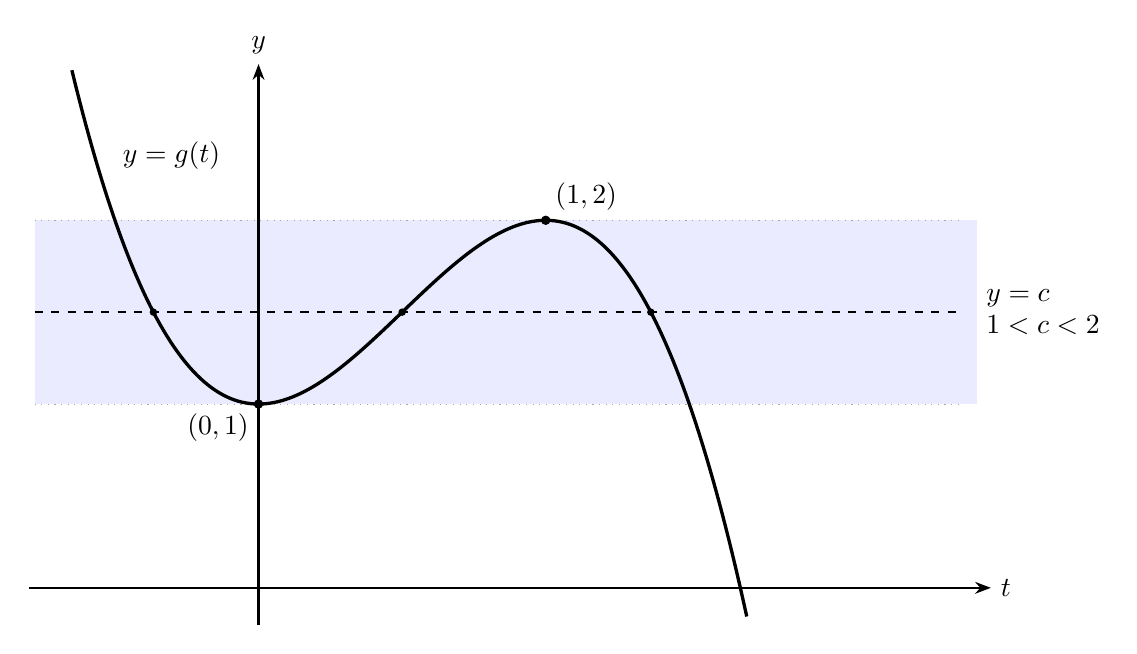
\begin{tikzpicture}
\pgfmathsetmacro{\tleft}{(1-sqrt(3))/2}
\pgfmathsetmacro{\tright}{(1+sqrt(3))/2}
\pgfmathsetmacro{\csample}{1.5}

\begin{axis}[
    width=13.8cm,
    height=8.7cm,
    axis lines=middle,
    axis line style={thick,-{Stealth[length=2mm]}},
    axis on top=true,
    xlabel={$t$},
    ylabel={$y$},
    xlabel style={at={(current axis.right of origin)},anchor=west},
    ylabel style={at={(current axis.above origin)},anchor=south,rotate=0},
    xmin=-0.8,
    xmax=2.55,
    ymin=-0.2,
    ymax=2.85,
    xtick=\empty,
    xticklabels={},
    ytick=\empty,
    yticklabels={},
    tick style={black},
    clip=false
]

% Shaded band 1<y<2
\path[fill=blue!8] (axis cs:-0.78,1) rectangle (axis cs:2.50,2);

% Boundary levels y=1 and y=2
\addplot[
    thin,
    dotted,
    gray!70,
    domain=-0.78:2.45,
    samples=2
] {1};

\addplot[
    thin,
    dotted,
    gray!70,
    domain=-0.78:2.45,
    samples=2
] {2};

% Representative line y=c
\addplot[
    thick,
    dashed,
    black,
    domain=-0.78:2.45,
    samples=2
] {\csample};

% The cubic
\addplot[
    very thick,
    black,
    domain=-0.65:1.7,
    samples=200
] {-2*x^3+3*x^2+1};

% Representative intersections for c=1.5
\fill[black] (axis cs:\tleft,1.5) circle (1.35pt);
\fill[black] (axis cs:0.5,1.5) circle (1.35pt);
\fill[black] (axis cs:\tright,1.5) circle (1.35pt);

% Turning points
\fill[black] (axis cs:0,1) circle (1.7pt);
\fill[black] (axis cs:1,2) circle (1.7pt);

% Labels
\node[left] at (axis cs:-0.1,2.35) {$y=g(t)$};
\node[below left] at (axis cs:0,1) {$(0,1)$};
\node[above right] at (axis cs:1,2) {$(1,2)$};

\node[anchor=west,align=left] at (axis cs:2.5,1.5)
    {$y=c$\\[-0.5pt] $1<c<2$};

\end{axis}
\end{tikzpicture}
% end q000616 figure F1
\end{djsSolutionFigure}
A horizontal line $y=c$ therefore crosses the graph of $y=g(t)$ three times precisely when it lies strictly between these stationary values. At $c=1$ or $c=2$, one intersection is repeated, so there are only two distinct points of tangency.

Hence the complete range is
\[
1<c<2
\]
the correct option is \textbf{C}.
% end q000616 solution
\end{djsSolution}
\end{enumerate}
\clearpage
\thispagestyle{djssolutions}
\vspace*{8pt}
\djsTopicLine{Trigonometry}
\begin{enumerate}[label=\textbf{\arabic*.},leftmargin=*,itemsep=0pt,start=17]
\questionitem[Trigonometry]
% begin q000671 stem
Find the complete set of real values of $k$ for which the equation
\[
2\cos^2 x - k\sin x + k = 0
\]
has exactly one solution in the range $0 \le x < 2\pi$.
% end q000671 stem

\par\vspace*{12pt}
\begin{tabularx}{\linewidth}{@{}>{\bfseries}l Y@{}}
A &
% begin q000671 choice A
$k < -4$ or $k > 0$
% end q000671 choice A
\\[0.8em]
B &
% begin q000671 choice B
$k \le -4$ or $k > 0$
% end q000671 choice B
\\[0.8em]
C &
% begin q000671 choice C
$k < -4$ or $k \ge 0$
% end q000671 choice C
\\[0.8em]
D &
% begin q000671 choice D
$k \le -4$ or $k \ge 0$
% end q000671 choice D
\\[0.8em]
E &
% begin q000671 choice E
$-4 < k < 0$
% end q000671 choice E
\\[0.8em]
F &
% begin q000671 choice F
$-4 \le k \le 0$
% end q000671 choice F
\\
\end{tabularx}

\begin{djsSolution}{B}
% begin q000671 solution
Let $s=\sin x$. Using $\cos^2x=1-\sin^2x$, the equation becomes
\[
2s^2+ks-k-2=0
\]
To factorise with the parameter $k$, group the terms to produce the common factor $s-1$:
\[
(2s^2-2)+(ks-k)=2(s-1)(s+1)+k(s-1)
\]
Hence
\[
(s-1)(2s+k+2)=0
\]
Therefore
\[
\sin x=1 \quad\text{or}\quad \sin x=-\frac{k+2}{2}
\]

Alternatively to factorising, using the quadratic formula:
\[
s=\frac{-k\pm\sqrt{k^2+8k+16}}{4}
=\frac{-k\pm(k+4)}{4}
\]
which gives the same two roots
\[
\sin x=1 \quad\text{or}\quad \sin x=-\frac{k+2}{2}
\]
The first equation always gives exactly one solution in the given range, namely
\[
x=\frac{\pi}{2}
\]
Therefore, for the original equation to have exactly one solution, the second equation
\[
\sin x=-\frac{k+2}{2}
\]
must either have no solutions, or give no additional solution

Since
\[
-1\leq \sin x\leq 1
\]
the second equation has no solutions when
\[
-\frac{k+2}{2}>1
\qquad\text{or}\qquad
-\frac{k+2}{2}<-1
\]
It also gives no additional solution when
\[
-\frac{k+2}{2}=1
\]
since this simply gives the same equation \(\sin x=1\)

However,
\[
-\frac{k+2}{2}=-1
\]
does not qualify, because \(\sin x=-1\) gives the additional solution
\[
x=\frac{3\pi}{2}
\]
The required cases are therefore
\[
-\frac{k+2}{2}>1,\qquad
-\frac{k+2}{2}<-1,
\qquad\text{or}\qquad
-\frac{k+2}{2}=1
\]
These give, respectively,
\[
k<-4,\qquad k>0,
\qquad\text{or}\qquad k=-4
\]
Combining them, the complete set is
\[
k\leq -4 \quad\text{or}\quad k>0
\]
so the correct option is \textbf{B}. \\[5pt]


\textit{Alternative Solution:} (testing the options)

The choices differ in whether the middle interval $-4<k<0$ is included and whether the endpoints $-4$ and $0$ are included. It is therefore enough to test one middle value and the two endpoints.

For $k=-2$, the quadratic in $s=\sin x$ becomes
\[
2s^2-2s=0
\]
so the two solutions are $\sin x=1$ and $\sin x=0$. These give
\[
x=\frac{\pi}{2}
\qquad\text{and}\qquad
x=0,\,\pi
\]
so there is not exactly one solution. This eliminates \textbf{E} and \textbf{F}.

For $k=-4$, the quadratic becomes
\[
2s^2-4s+2=0
\]
which factorises as
\[
2(s-1)^2=0
\]
so both roots coincide at $\sin x=1$. Hence there is exactly one solution
\[
x=\frac{\pi}{2}
\]
Thus $-4$ must be included, eliminating \textbf{A} and \textbf{C}.

For $k=0$, the quadratic becomes
\[
2s^2-2=0
\]
so the two solutions are $\sin x=1$ and $\sin x=-1$. These give
\[
x=\frac{\pi}{2}
\qquad\text{and}\qquad
x=\frac{3\pi}{2}
\]
so there are two solutions. Hence $0$ must be excluded, eliminating \textbf{D}. \\The remaining option is \textbf{B}.
% end q000671 solution
\end{djsSolution}
\end{enumerate}
\clearpage
\thispagestyle{djssolutions}
\vspace*{8pt}
\djsTopicLine{Polynomials}
\begin{enumerate}[label=\textbf{\arabic*.},leftmargin=*,itemsep=0pt,start=18]
\questionitem[Polynomials]
% begin q000532 stem
Let $f(x)=x^4+ax^2+b$, where $a$ and $b$ are real constants.

The minimum value of $f(x)$ is $-4$, and the equation $f(x)=0$ has exactly three distinct real solutions.

What is the value of $a$ and the value of $b$?
% end q000532 stem

\par\vspace*{12pt}
\begin{tabularx}{\linewidth}{@{}>{\bfseries}l Y@{}}
A &
% begin q000532 choice A
$a=-4,\,b=-4$
% end q000532 choice A
\\[0.8em]
B &
% begin q000532 choice B
$a=-4,\,b=0$
% end q000532 choice B
\\[0.8em]
C &
% begin q000532 choice C
$a=-2,\,b=0$
% end q000532 choice C
\\[0.8em]
D &
% begin q000532 choice D
$a=0,\,b=-4$
% end q000532 choice D
\\[0.8em]
E &
% begin q000532 choice E
$a=4,\,b=-4$
% end q000532 choice E
\\[0.8em]
F &
% begin q000532 choice F
$a=4,\,b=0$
% end q000532 choice F
\\
\end{tabularx}

\begin{djsSolution}{B}
% begin q000532 solution
Let $u=x^2$, so $u\geq 0$. The equation $f(x)=0$ becomes
\[
u^2+au+b=0
\]
A positive solution $u=r$ produces the two distinct real solutions $x=\sqrt r$ and $x=-\sqrt r$, whereas $u=0$ produces only the single solution $x=0$. Since there are exactly three distinct real solutions in $x$, the two relevant solutions in $u$ must therefore be $u=0$ and $u=r$ for some $r>0$.

Substituting $u=0$ gives $b=0$. The equation then factorises as
\[
u^2+au=u(u+a)=0
\]
so its other solution is $u=-a$. As this solution is positive, $a<0$.

Now complete the square:
\[
f(x)=u^2+au=\left(u+\frac a2\right)^2-\frac{a^2}{4}
\]
Because $a<0$, the value $u=-\dfrac a2$ is positive and hence is attainable by an appropriate value of $x$.

Therefore, from the completed square form, the minimum value is $-\dfrac{a^2}{4}$. Thus
\[
-\frac{a^2}{4}=-4
\]
so $a^2=16$. The condition $a<0$ selects $a=-4$, and $b=0$. Hence the correct option is \textbf{B}. \\

\textit{Alternative Solution:}

$f(x)$ depends only on $x^2$. Thus the function $f(x)$ is an even function, since $f(-x)=f(x)$. 

Recall that even functions are exactly those functions with graphs for which the $y$-axis is a line of symmetry.

Consequently, every non-zero root occurs with its reflection in the $y$-axis: if $x=c$ is a root, then $x=-c$ is also a root. An odd number of distinct roots is therefore possible only if $x=0$ is also a root. 

Hence $f(0)=0$. But $f(0)=b$ so $b=0$.

Since the minimum is negative we must have $a<0$, as otherwise:
\[
f(x) = x^4+ax^2\geq0
\]for all $x$. Completing the square gives
\[
f(x)=\left(x^2+\frac a2\right)^2-\frac{a^2}{4}
\]
The squared term can equal zero because $-a/2>0$. The minimum is therefore $-a^2/4=-4$, giving $a=-4$. Together with $b=0$, this again gives \textbf{B}.
% end q000532 solution
\end{djsSolution}
\end{enumerate}
\clearpage
\thispagestyle{djssolutions}
\vspace*{8pt}
\djsTopicLine{Functions \& Graphs}
\begin{enumerate}[label=\textbf{\arabic*.},leftmargin=*,itemsep=0pt,start=19]
\questionitem[Functions \& Graphs]
% begin q000605 stem
For a positive real constant $k$, the equation

\[
\left|x^2-4x+3\right|=kx
\]

has exactly three distinct real solutions.

Find the complete set of possible values of $k$.
% end q000605 stem

\par\vspace*{12pt}
\begin{tabularx}{\linewidth}{@{}>{\bfseries}l Y@{}}
A &
% begin q000605 choice A
There are no such positive values of $k$.
% end q000605 choice A
\\[0.8em]
B &
% begin q000605 choice B
$0<k<4-2\sqrt{3}$
% end q000605 choice B
\\[0.8em]
C &
% begin q000605 choice C
$k=4-2\sqrt{3}$
% end q000605 choice C
\\[0.8em]
D &
% begin q000605 choice D
$k=4+2\sqrt{3}$
% end q000605 choice D
\\[0.8em]
E &
% begin q000605 choice E
$k=4-2\sqrt{3}$ or $k=4+2\sqrt{3}$
% end q000605 choice E
\\
\end{tabularx}

\begin{djsSolution}{C}
% begin q000605 solution
Write
\[
q(x)=x^2-4x+3=(x-1)(x-3)
\]
The quadratic $q(x)$ is negative between its roots $1$ and $3$. The absolute value reflects this part above the $x$-axis, so
\[
\left|x^2-4x+3\right|=
\begin{cases}
x^2-4x+3, & x\leq 1\text{ or }x\geq 3,\\
-x^2+4x-3, & 1\leq x\leq 3.
\end{cases}
\]

\begin{djsSolutionFigure}
% begin q000605 figure F1
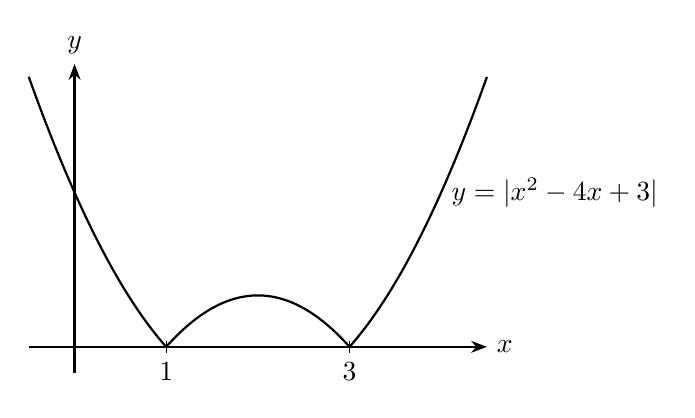
\begin{tikzpicture}
\begin{axis}[
    width=7.4cm,
    height=5.5cm,
    axis lines=middle,
    axis line style={thick,-{Stealth[length=2mm]}},
    xlabel={$x$},
    ylabel={$y$},
    xlabel style={at={(current axis.right of origin)},anchor=west},
    ylabel style={at={(current axis.above origin)},anchor=south},
    xmin=-0.5,
    xmax=4.5,
    ymin=-0.5,
    ymax=5.5,
    xtick={1,3},
    ytick=\empty,
    tick style={black},
    clip=false,
    clip marker paths=false
]
\addplot[thick,black,domain=-0.5:1,samples=80]
    {x^2-4*x+3};
\addplot[thick,black,domain=1:3,samples=100]
    {-x^2+4*x-3};
\addplot[thick,black,domain=3:4.5,samples=80]
    {x^2-4*x+3}
    node[pos=0.58, right] {$y=|x^2-4x+3|$};
\end{axis}
\end{tikzpicture}
% end q000605 figure F1
\end{djsSolutionFigure}

For \(k>0\), the graph shows that the line \(y=kx\) meets each of the two upward-facing branches exactly once. Thus these branches always contribute two solutions:

\begin{djsSolutionFigure}
% begin q000605 figure F4
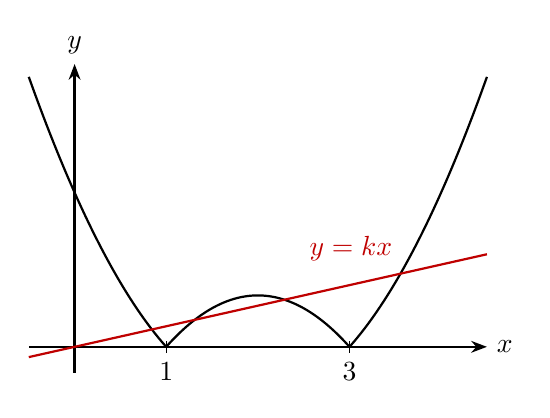
\begin{tikzpicture}
\begin{axis}[
    width=7.4cm,
    height=5.5cm,
    axis lines=middle,
    axis line style={thick,-{Stealth[length=2mm]}},
    xlabel={$x$},
    ylabel={$y$},
    xlabel style={at={(current axis.right of origin)},anchor=west},
    ylabel style={at={(current axis.above origin)},anchor=south},
    xmin=-0.5,
    xmax=4.5,
    ymin=-0.5,
    ymax=5.5,
    xtick={1,3},
    ytick=\empty,
    tick style={black},
    clip=false,
    clip marker paths=false
]
\addplot[thick,black,domain=-0.5:1,samples=80]
    {x^2-4*x+3};
\addplot[thick,black,domain=1:3,samples=100]
    {-x^2+4*x-3};
\addplot[thick,black,domain=3:4.5,samples=80]
    {x^2-4*x+3};

\addplot[thick,red!75!black,domain=-0.5:4.5,samples=2]
    {0.4*x}
    node[pos=0.82, above left=1pt, text=red!75!black] {$y=kx$};
\end{axis}
\end{tikzpicture}
% end q000605 figure F4
\end{djsSolutionFigure}

For there to be exactly three distinct solutions altogether, the line must therefore meet the central arch exactly once. This occurs when \(y=kx\) is tangent to the central arch.

We therefore need exactly one further solution on the central arch. There,
\[
kx=-x^2+4x-3
\]
so
\[
x^2-(4-k)x+3=0
\]
The line must be tangent to the arch, giving a repeated root. Equivalently, the discriminant must be zero:
\[
(4-k)^2-12=0
\]
Hence
\[
4-k=\pm2\sqrt3
\]
and the two candidates are
\[
k=4-2\sqrt3\quad\text{or}\quad k=4+2\sqrt3
\]

Care is needed because the central formula is valid only for $1\leq x\leq3$. 

The repeated root of a quadratic with zero discriminant is given by $-\dfrac{b}{2a}$. In this case:
\[
x=\frac{4-k}{2}
\]
For $k=4-2\sqrt3$, this gives $x=\sqrt3$, which lies between $1$ and $3$. This is the required third intersection:

\begin{djsSolutionFigure}
% begin q000605 figure F2
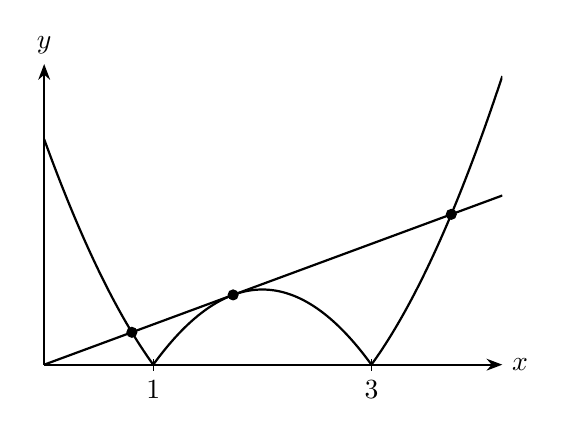
\begin{tikzpicture}
\pgfmathsetmacro{\ksmall}{4-2*sqrt(3)}
\pgfmathsetmacro{\xtan}{sqrt(3)}
\pgfmathsetmacro{\ytan}{4*sqrt(3)-6}
\pgfmathsetmacro{\xleft}{6-3*sqrt(3)}
\pgfmathsetmacro{\yleft}{\ksmall*\xleft}
\pgfmathsetmacro{\xright}{2+sqrt(3)}
\pgfmathsetmacro{\yright}{\ksmall*\xright}

\begin{axis}[
    width=7.4cm,
    height=5.4cm,
    axis lines=left,
    axis line style={thick,-{Stealth[length=2mm]}},
    xlabel={$x$},
    ylabel={$y$},
    xlabel style={at={(current axis.right of origin)},anchor=west},
    ylabel style={at={(current axis.above origin)},anchor=south, rotate=270},
    xmin=0,
    xmax=4.2,
    ymin=0,
    ymax=4,
    xtick={1,3},
    ytick=\empty,
    tick style={black},
    clip=true,
    clip marker paths=false
]

\addplot[thick,black,domain=0:1,samples=70]
    {x^2-4*x+3};

\addplot[thick,black,domain=1:3,samples=100]
    {-x^2+4*x-3};

\addplot[thick,black,domain=3:4.2,samples=70]
    {x^2-4*x+3};

\addplot[thick,black,domain=0:4.2,samples=2]
    {\ksmall*x};

\addplot[only marks,mark=*,mark size=1.8pt,black]
    coordinates {
        (\xleft,\yleft)
        (\xtan,\ytan)
        (\xright,\yright)
    };

\node[below] at (axis cs:\xtan,0) {$\sqrt{3}$};

\end{axis}
\end{tikzpicture}
% end q000605 figure F2
\end{djsSolutionFigure}

For $k=4+2\sqrt3$, the repeated root is $x=-\sqrt3$. This is a tangency to the extension of the central parabola, not to the part used in the absolute-value graph. There is therefore no central intersection for this value of $k$:

\begin{djsSolutionFigure}
% begin q000605 figure F3
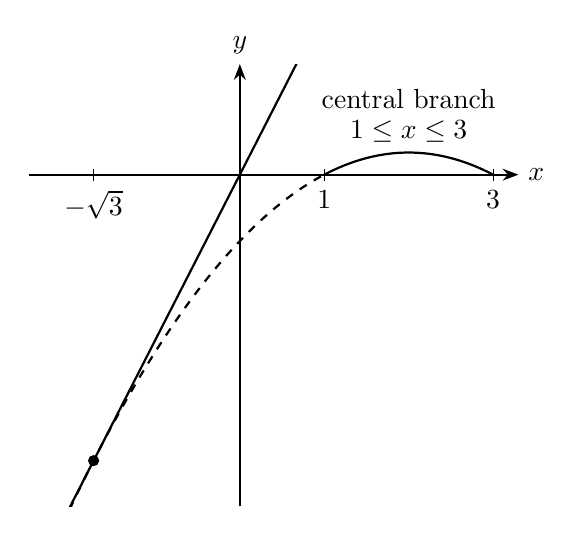
\begin{tikzpicture}
\pgfmathsetmacro{\klarge}{4+2*sqrt(3)}
\pgfmathsetmacro{\xT}{-sqrt(3)}
\pgfmathsetmacro{\yT}{-4*sqrt(3)-6}

\begin{axis}[
    width=7.8cm,
    height=7.2cm,
    axis lines=middle,
    axis line style={thick,-{Stealth[length=2mm]}},
    xlabel={$x$},
    ylabel={$y$},
    xlabel style={at={(current axis.right of origin)},anchor=west},
    ylabel style={at={(current axis.above origin)},anchor=south},
    xmin=-2.5,
    xmax=3.3,
    ymin=-15,
    ymax=5,
    xtick={\xT,1,3},
    xticklabels={$-\sqrt{3}$,$1$,$3$},
    ytick=\empty,
    tick style={black},
    clip=true,
    clip marker paths=false
]

\addplot[dashed,thick,black,domain=-2.5:1,samples=140]
    {-x^2+4*x-3};

\addplot[thick,black,domain=1:3,samples=100]
    {-x^2+4*x-3}
    node[pos=0.5,above,align=center]
    {central branch\\[-1pt]$1\leq x\leq 3$};

\addplot[thick,black,domain=-2.5:3.3,samples=2]
    {\klarge*x}
    node[pos=0.68,above,sloped] {$y=(4+2\sqrt{3})x$};

\addplot[only marks,mark=*,mark size=1.8pt,black]
    coordinates {(\xT,\yT)};

\end{axis}
\end{tikzpicture}
% end q000605 figure F3
\end{djsSolutionFigure}

Consequently, the complete set of possible values is $k=4-2\sqrt3$, so the correct option is \textbf{C}.
% end q000605 solution
\end{djsSolution}
\end{enumerate}
\clearpage
\thispagestyle{djssolutions}
\vspace*{8pt}
\djsTopicLine{Geometry}
\begin{enumerate}[label=\textbf{\arabic*.},leftmargin=*,itemsep=0pt,start=20]
\questionitem[Geometry]
% begin q000600 stem
A circle passes through the vertices of a right-angled triangle $ABC$, where angle $ABC = 90^\circ$, $AB = 12\text{ cm}$, and $BC = 16\text{ cm}$.

A line is drawn through $A$ parallel to $BC$. 

This line intersects the tangent to the circle at $B$ at the point $P$.

What is the length of $AP$?
% end q000600 stem

\par\vspace*{12pt}
\begin{tabularx}{\linewidth}{@{}>{\bfseries}l Y@{}}
A &
% begin q000600 choice A
$7.2\text{ cm}$
% end q000600 choice A
\\[0.8em]
B &
% begin q000600 choice B
$8\text{ cm}$
% end q000600 choice B
\\[0.8em]
C &
% begin q000600 choice C
$9\text{ cm}$
% end q000600 choice C
\\[0.8em]
D &
% begin q000600 choice D
$9.6\text{ cm}$
% end q000600 choice D
\\[0.8em]
E &
% begin q000600 choice E
$10\text{ cm}$
% end q000600 choice E
\\[0.8em]
F &
% begin q000600 choice F
$16\text{ cm}$
% end q000600 choice F
\\
\end{tabularx}

\begin{djsSolution}{C}
% begin q000600 solution
A diagram with the two constructed lines is shown below:

\begin{djsSolutionFigure}
% begin q000600 figure F1
\begin{tikzpicture}[x=0.4cm,y=0.4cm,line cap=round,line join=round]
\path[use as bounding box] (-11.5,-6.5) rectangle (19.5,17.5);
\clip (-11.5,-6.5) rectangle (19.5,17.5);

\coordinate (A) at (0,12);
\coordinate (B) at (0,0);
\coordinate (C) at (16,0);
\coordinate (P) at (-9,12);
\coordinate (O) at (8,6);
\def\radius{10}
\pgfmathsetmacro{\ttforward}{4/3}
\coordinate (Tright) at ($(P)!\ttforward!(B)$);

\draw[thick,gray!70] (O) circle (\radius);
\draw[thick,black,
  postaction={decorate,decoration={markings,
  mark=at position 0.5 with {\arrow{Stealth[length=2mm]}}}}]
  (P) -- (A);
\draw[thick,black] (P) -- (Tright);
\draw[thick,black] (A) -- (B);
\draw[thick,black,
  postaction={decorate,decoration={markings,
  mark=at position 0.5 with {\arrow{Stealth[length=2mm]}}}}]
  (B) -- (C);
\draw[thick,black] (C) -- (A);

\path (A) -- (B) node[midway,right=3pt] {$12\text{ cm}$};
\path (B) -- (C) node[midway,below=4pt] {$16\text{ cm}$};

\foreach \Q in {A,B,C,P}{\fill (\Q) circle (1.4pt);}
\node[right, yshift=3pt] at (A) {$A$};
\node[below left] at (B) {$B$};
\node[right] at (C) {$C$};
\node[above left] at (P) {$P$};
\end{tikzpicture}
% end q000600 figure F1
\end{djsSolutionFigure}

Since $PB$ is tangent to the circle at $B$ and $BA$ is a chord, the alternate segment theorem gives
\[
\angle PBA=\angle BCA
\]

Also, $AP$ is parallel to $BC$. Since $AB$ is perpendicular to $BC$, it is also perpendicular to $AP$, so
\[
\angle PAB=\angle ABC=90^\circ
\]

The remaining angles are therefore equal as well, because the angles in each triangle sum to $180^\circ$. The corresponding angles are marked with the same colour and symbol in the diagram below.

\begin{djsSolutionFigure}
% begin q000600 figure F2
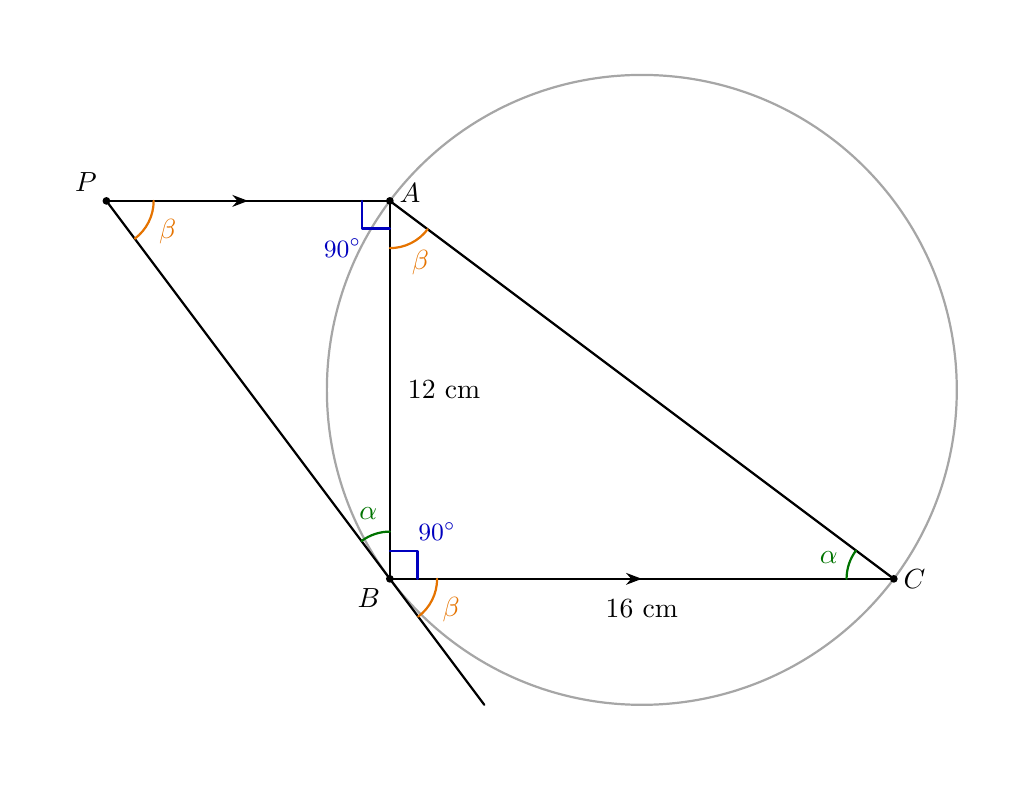
\begin{tikzpicture}[x=0.4cm,y=0.4cm,line cap=round,line join=round]
\path[use as bounding box] (-11.5,-6.5) rectangle (19.5,17.5);
\clip (-11.5,-6.5) rectangle (19.5,17.5);

\coordinate (A) at (0,12);
\coordinate (B) at (0,0);
\coordinate (C) at (16,0);
\coordinate (P) at (-9,12);
\coordinate (O) at (8,6);
\def\radius{10}
\pgfmathsetmacro{\ttforward}{4/3}
\coordinate (Tright) at ($(P)!\ttforward!(B)$);

\draw[thick,gray!70] (O) circle (\radius);
\draw[thick,black,
  postaction={decorate,decoration={markings,
  mark=at position 0.5 with {\arrow{Stealth[length=2mm]}}}}]
  (P) -- (A);
\draw[thick,black] (P) -- (Tright);
\draw[thick,black] (A) -- (B);
\draw[thick,black,
  postaction={decorate,decoration={markings,
  mark=at position 0.5 with {\arrow{Stealth[length=2mm]}}}}]
  (B) -- (C);
\draw[thick,black] (C) -- (A);

\path (A) -- (B) node[midway,right=3pt] {$12\text{ cm}$};
\path (B) -- (C) node[midway,below=4pt] {$16\text{ cm}$};

\foreach \Q in {A,B,C,P}{\fill (\Q) circle (1.4pt);}
\node[right, yshift=3pt] at (A) {$A$};
\node[below left] at (B) {$B$};
\node[right] at (C) {$C$};
\node[above left] at (P) {$P$};

\pic["$\alpha$",draw=green!45!black,text=green!45!black,
  thick,angle radius=6mm,angle eccentricity=1.45]
  {angle=A--B--P};
\pic["$\alpha$",draw=green!45!black,text=green!45!black,
  thick,angle radius=6mm,angle eccentricity=1.45]
  {angle=A--C--B};

\pic[draw=blue!75!black,thick,angle radius=3.5mm]
  {right angle=P--A--B};
\pic[draw=blue!75!black,thick,angle radius=3.5mm]
  {right angle=C--B--A};
\node[text=blue!75!black,font=\small,xshift=-6mm,yshift=-6mm]
  at (A) {$90^\circ$};
\node[text=blue!75!black,font=\small,xshift=6mm,yshift=6mm]
  at (B) {$90^\circ$};

\pic["$\beta$",draw=orange!90!black,text=orange!90!black,
  thick,angle radius=6mm,angle eccentricity=1.45]
  {angle=B--P--A};
\pic["$\beta$",draw=orange!90!black,text=orange!90!black,
  thick,angle radius=6mm,angle eccentricity=1.45]
  {angle=B--A--C};
\pic["$\beta$",draw=orange!90!black,text=orange!90!black,thick,angle radius=6mm,angle eccentricity=1.45]{angle=Tright--B--C};
\end{tikzpicture}
% end q000600 figure F2
\end{djsSolutionFigure}

Thus triangles $PBA$ and $ABC$ are similar. In triangle $PBA$, the vertices $P,B,A$ correspond respectively to $A,C,B$ in triangle $ABC$. Therefore $AB$ in triangle $PBA$ corresponds to $BC$ in triangle $ABC$, while $PA$ corresponds to $AB$ in triangle $ABC$.

The scale factor from triangle $ABC$ to triangle $PBA$ is consequently
\[
\frac{12}{16}=\frac34
\]

Since $PA$ corresponds to the $12\text{ cm}$ side $AB$ in triangle $ABC$,
\[
PA=\frac34\times12=9\text{ cm}
\]

Hence the correct option is \textbf{C}.
% end q000600 solution
\end{djsSolution}
\end{enumerate}
\end{document}
